\section{Appendix}
In this supplementary document, we first present additional information about our dataset, evaluation setting, implementation details in \cref{sec:supp_data}. We then elaborate on technical details of our methods in \cref{sec:supp_method}. Additional results of the two return mask segmentation, more quantitative and qualitative results are provided in \cref{sec:supp_results}.

\subsection{Datasets and implementation details}
\label{sec:supp_data}
\paragraph{Town dataset}
To simulate \textit{TownReal} dataset, we approximate a diverged beam profile using 37 subrays and the divergence angle $\gamma_0 = 2 $~mrad~\cite{glennie2012calibration}. We use the subray distribution proposed from~\cite{winiwarter2022virtual}~(\cf \cref{fig:diverged_ray}). The dataset is shown in~\cref{fig:supp_town_dataset}. 

\paragraph{Waymo dataset}
We use the following 4 scenes~(\cf \cref{fig:supp_waymo_dataset}) that are mostly static from \textit{Waymo}~\cite{sun2020scalability} dataset 


\begin{table}[!h]
    \setlength{\tabcolsep}{6pt}
    \renewcommand{\arraystretch}{1.2}
	\centering
	\resizebox{0.8\columnwidth}{!}{
    \begin{tabular}{l|c}
    \toprule
    & Scene ID \\
    \midrule
    Scene 1 & 10017090168044687777\_6380\_000\_6400\_000 \\
    Scene 2 & 10096619443888687526\_2820\_000\_2840\_000 \\
    Scene 3 & 10061305430875486848\_1080\_000\_1100\_000 \\
    Scene 4 & 10275144660749673822\_5755\_561\_5775\_561 \\
    \bottomrule
    \end{tabular}
    }
\end{table}

\paragraph{\textit{Waymo NVS} setting} 
We simulate the new trajectory by shifting the sensor by [1.5, 1.5, 0.5] meters (see \cref{fig:supp_waymo_dataset}), yielding an overall displacement of ${\approx}2.18$ meters. This displacement magnitude corresponds to the requirements of various tasks, such as lane changes or adapting the sensor rig from a car to a truck. Moreover, our displacement from the trajectory is similar~\cite{Yang_2023_unisim} or even larger~\cite{Ost_2022_CVPR} than used in prior NVS works. Nevertheless, we run additional experiments by varying the displacements and report results in \cref{tab:rebuttaL_nvs}. NFL consistently outperforms baseline methods under different settings, and the improvement is more pronounced under large displacements.

\begin{table}[t]
    \setlength{\tabcolsep}{6pt}
    \renewcommand{\arraystretch}{1.2}
	\centering
	\resizebox{1.0\columnwidth}{!}{
    \begin{tabular}{c|ccccc}
    \toprule
     & i-NGP & DS-NeRF & URF & LiDARsim & Ours \\
    \midrule
    (0.5, 0.5, 0.5)  & 7.0 / 14.4 & 7.0 / 16.0 & 9.0 / 19.6 & 16.1 / 33.1 & \textbf{5.4} / \textbf{13.0} \\
    (1.5, 1.5, 1.0)  & 8.4 / 17.6 & 7.8 / 18.5 & 11.0 / 27.5 & 16.5 / 37.9 & \textbf{5.8} / \textbf{14.3}  \\
    (2.5, 2.5, 1.5)  & 11.6 / 28.0 & 9.3 / 22.8 & 13.9 / 35.5 & 17.2 / 46.3 & \textbf{6.4} / \textbf{18.4} \\
    \bottomrule
    \end{tabular}
    }
    \caption{Varying the displacement on \textit{Waymo NVS} dataset. Numbers are reported as \textit{MedAE} / \textit{CD} [cm].}
    \label{tab:rebuttaL_nvs}
\end{table}

\paragraph{Point cloud registration task}
We utilize 49 paired consecutive frames per scene, with a relative displacement of ${\approx}1$ meter. \textit{TE} is reported in centimeters and \textit{RE} is reported in degrees.


\subsection{Implementation details}
\paragraph{Our method.}
Our model is implemented based on \emph{torch-ngp}~\cite{torch-ngp,muller2022instant} and can be trained on a single RTX 3090 GPU. During training we minimize \refpaper{eq:loss_function} using the Adam~\cite{kingma2014adam} optimiser, with an initial learning rate of 0.005 which linearly decays to 0.0005 towards the end of training. We clip the gradient magnitudes of all parameters to 1.0 to stabilize the optimisation. In the first stage, we sample $N^c = 768$ points and in the second stage $N^f=64$ points for each ray. The window size $\epsilon$ for volume rendering is set to 0.8 m, and the buffer value $\xi$ between two returns is set to 2 m. The weights in the loss function, i.e., $\lambda_e$, $\lambda_d$, and $\lambda_s$, are set to 50, 0.15, and 0.15, respectively.

\begin{figure}[t]
\centering
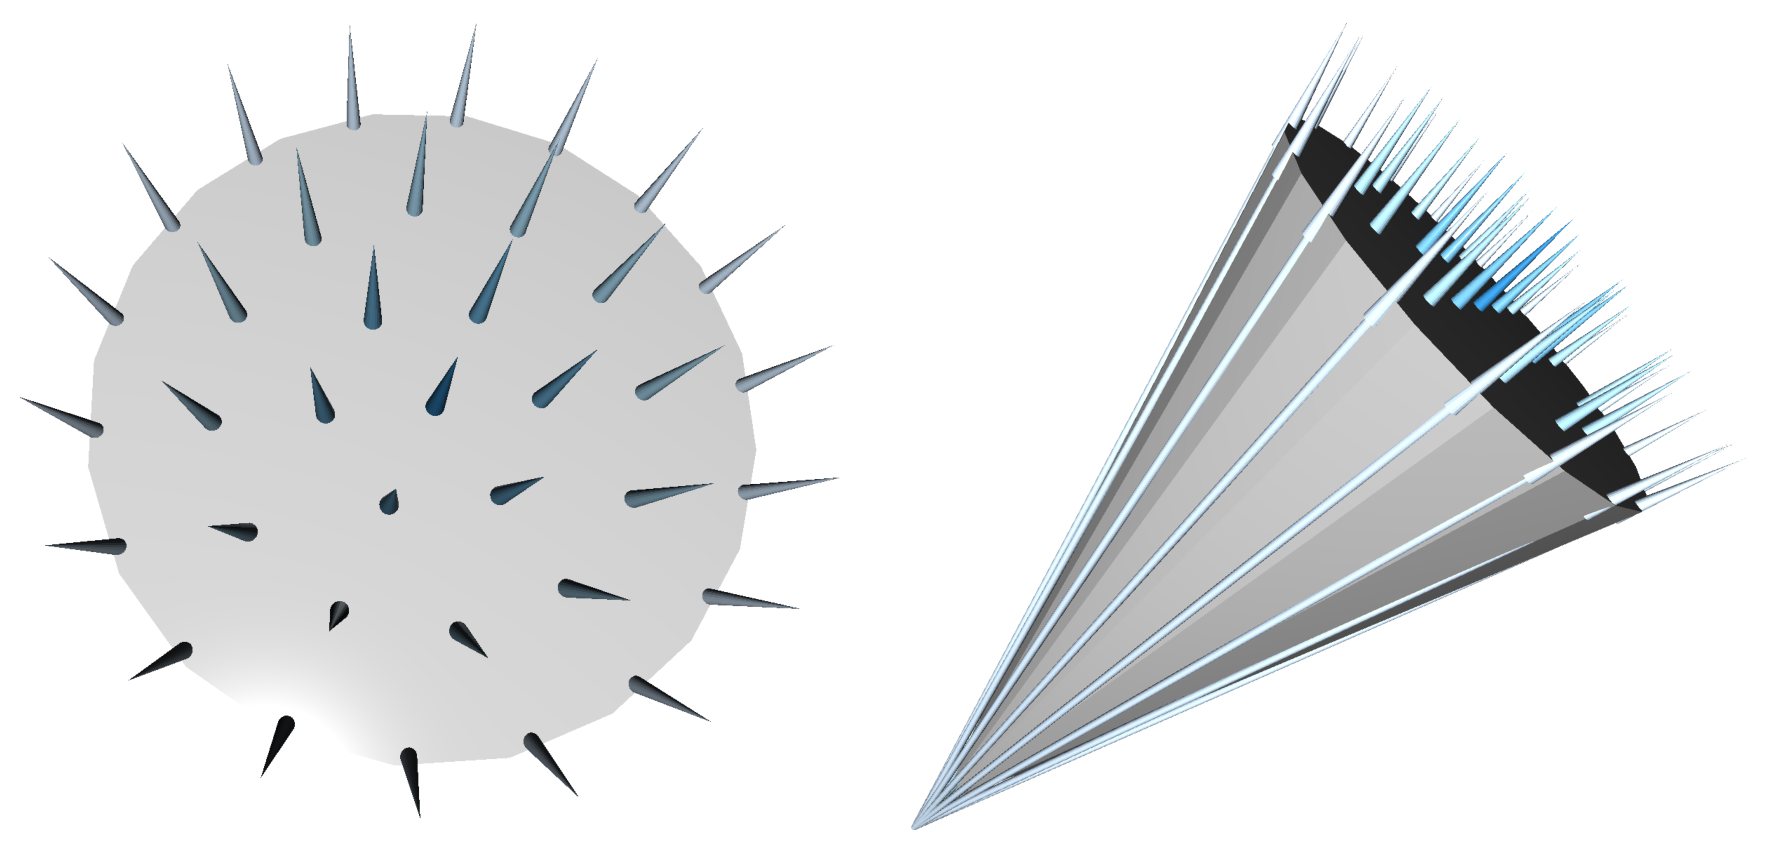
\includegraphics[width=0.6\columnwidth]{supp/images/diverged_beam.pdf}
\caption{Example diverged beam profile approximated via 37 diverged rays.}
\label{fig:diverged_ray}
\end{figure}

\paragraph{LiDARsim.}
Because the original implementation is not publicly available, we re-implemented LiDARsim~\cite{manivasagam2020lidarsim} following the paper as close as possible. Specifically, for all points in the training set, we first estimate pointwise normal vectors using all points within a 20 cm radius ball. Then, we apply voxel down-sampling~\cite{tang2022torchsparse} with a voxel size of 4 cm and reconstruct a disk surfel\footnote{We use the implementation from Point-Cloud-Utils~\cite{point-cloud-utils} library.} for each point. Here, the input point represents the disk center and it orientation is defined by the estimated normal vector. At inference time, we perform ray-surfel intersection to determine the intersection points. We empirically observed that LiDARsim's~\cite{manivasagam2020lidarsim} performance is sensitive to the selected surfel radius. Therefore, we have experimented with both a distance-dependent and fixed surfel radius and found that fixed surfel radius of 6 cm and 12 cm for \textit{Waymo} and \textit{Town} dataset, respectively lead to best range accuracy. To enable second range estimation, we augment LiDARsim with a diverged beam profile approximated using 7 rays. To obtain the second return mask, we consider a LiDAR beam to have two returns if the maximum range difference between all subrays is larger than a threshold\footnote{Sensor-specific parameter, 2 m on \textit{Waymo} dataset.}. The first return is defined as the closest ray-surfel intersection, while the second return is the nearest one that is at least two meters away. To train the ray drop module, we utilize 40k samples from the Waymo dataset~\cite{sun2020scalability}, and only apply this module after the ray-surfel intersection to refine the ray drop patterns. Please see~\cref{fig:supp_lidarsim_raydrop} for more qualitative results. 


\paragraph{Other NeRF methods.}
We also use \emph{torch-ngp}~\cite{torch-ngp} codebase to implement other methods, using the same network and sampling configurations as used in ours. To estimate the range, we remove the radiance MLP and instead, apply volume rendering of the sampled $\zeta$ along the ray.  For DS-NeRF~\cite{deng2021depth} and URF~\cite{rematas2021urban}, we replace their positional encoding with a hash-grid~\cite{muller2022instant} to facilitate a fair comparison with i-NGP~\cite{muller2022instant}. Moreover, we substitute the original L2 loss with the L1 loss, as it results in better performance. Finally, we follow the original paper and augment DS-NeRF~\cite{deng2021depth} and URF~\cite{rematas2021urban} with the ray distribution loss and line-of-sight loss, respectively, to regularise the underlying geometry. 


\subsection{Methodology and loss functions}
\label{sec:supp_method}
\paragraph{First range estimation}
If the maximum weight at the first stage $w_p^c$ is below a predefined threshold $\eta=0.1$, we assume that the network is uncertain about the reconstruction and the resulting range estimate may be inaccurate. In these cases, we only apply the coarse stage volume rendering and directly estimate the range as: $\zeta = \sum_{j=1}^{N^c} w_j^c \cdot \zeta_j$. 

\paragraph{Range reconstruction loss}
For coarse range, we impose a Gaussian distribution around the ground truth $\hat{\zeta}$ and we anneal the standard deviation $\delta$ during training, the annealing procedure is defined as:
\begin{equation}
    \delta_k = \delta_{\max} \left(\frac{\delta_{\min}}{\delta_{\max}}\right)^{k / k_{\max}}
\end{equation}
where $k$ denotes the iteration number, $k_{\max}$ is the maximum iteration, and $\delta_{\max}$ and $\delta_{\min}$ correspond to empirically determined bounds for the standard deviation. The annealing parameters $\delta_{\min}$ and $\delta_{\max}$ are set to 0.25/0.3 and 1.2/1.6, respectively, for the \textit{Town} and \textit{Waymo} datasets. The maximum iteration $k_{\max}$ is set to 16000/24000 for the \textit{Town} and \textit{Waymo} datasets. 
The ground truth weight $\hat{w}_j$ is computed as:
\begin{equation}
    \hat{w}_j = \int_{\zeta_j}^{\zeta_{j+1}} \frac{1}{\delta\sqrt{2\pi}}\exp\left(-\frac{(x - \hat{\zeta})^2}{2\delta^2}\right) \; dx.
\end{equation}


\subsection{Additional results}
\label{sec:supp_results}
\begin{figure}[!t]
    \centering
        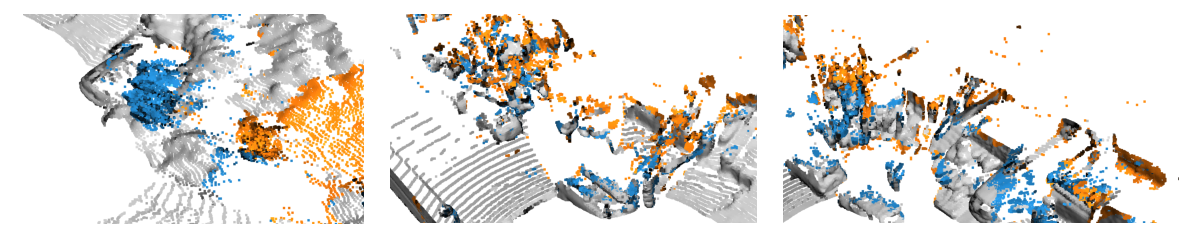
\includegraphics[width=1.0\textwidth]{content/main/images/rebuttal_secondary_return.pdf}
        \caption{Rendered secondary returns are color-coded in {\setlength{\fboxsep}{0pt}\colorbox{sdpoints}{yellow}}.}
    \label{fig:rebuttal_second_return}
\end{figure}
\paragraph{Runtime analysis}
Our \textit{central ray} version takes 4.1 ms per frame to render the single returns on an RTX 3090 GPU, while other NeRF-style methods require 2.4 ms. Only around $10\%$ of rays have second returns, resulting in low computational overhead. While our \textit{diverged beam} incurs additional costs due to querying diverged rays, it can be disabled if needed, without compromising first return performance (\cf Tab. 1). Our re-implementation of LiDARsim achieves 10 Hz runtime, but could be further improved using accelerated ray-tracing, \eg OptiX. Note that all methods already match or even (greatly) exceed the normal LiDAR measurement frequency (${\approx}10$ Hz). 

\paragraph{Ray drop modelling}
There clearly is a link between ray drops and beam divergence. However, we found that modeling it through the beam feature yields worse performance, possibly because $\rayfeat$ uses $\rangefeat$, which encodes the statistics of returns and is less meaningful for dropped rays. In future work, beam divergence could instead be incorporated through Intergrated Positional Encoding~\cite{barron2023zipnerf} to model ray drops.

\paragraph{Two return mask prediction}
\begin{figure}[t]
\centering
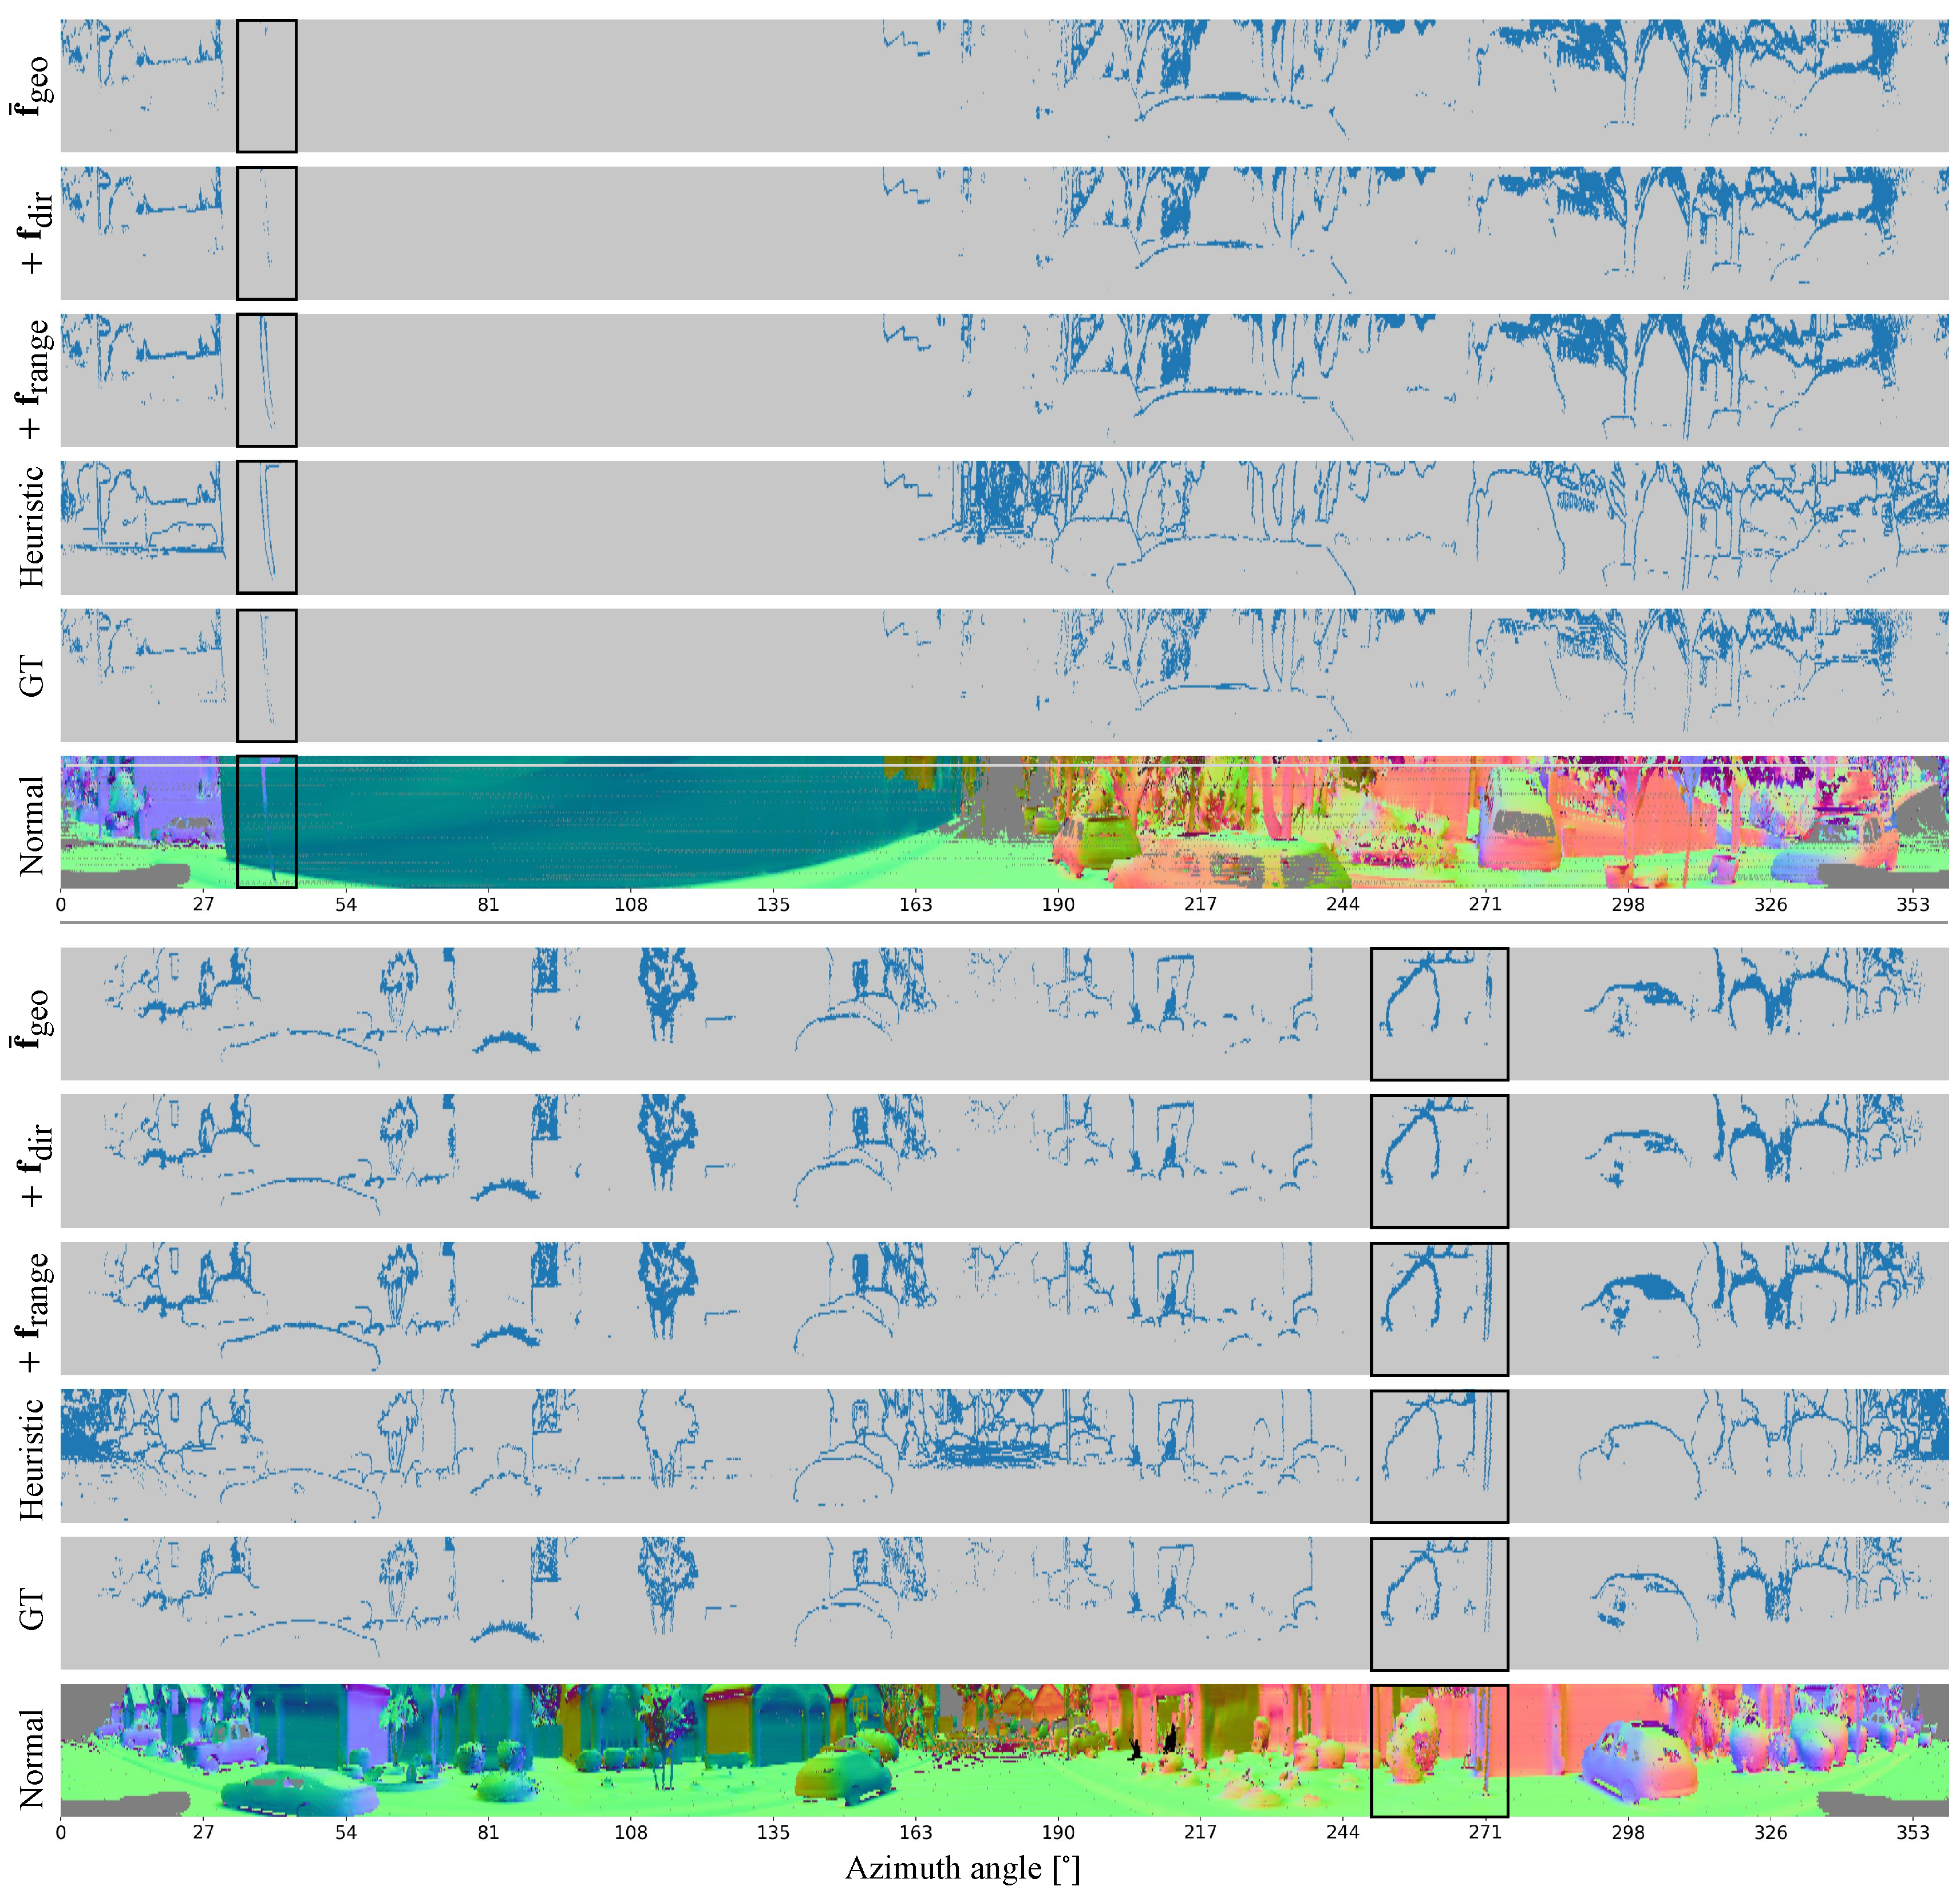
\includegraphics[width=1.0\textwidth]{content/supp/images/ablate_two_return_mask.pdf}

\caption{Qualitative results of two return mask segmentation.}
\label{fig:supp_ablate_two_return_mask}

\end{figure}
We conduct an ablation study to investigate different design choices for predicting the two return mask and summarize the results in~\cref{tab:ablate_two_return_mask}. We observe that concatenating the range feature $\rangefeat$ with the beam feature $\rayfeat$ improves the segmentation recall and, consequently, the second range estimation. In addition to predicting the two return mask from the beam feature, we experiment with a simple heuristic-based baseline that thresholds the depth standard deviation of sub-rays. Specifically, we considered a LiDAR beam to have two returns if the standard deviation is above 30\footnote{Empirically determined as it leads to the best Intersection-of-Union score.} cm. However, as shown in Table~\ref{tab:ablate_two_return_mask}, this approach achieves limited success and performs much worse than the learned methods. More qualitative results are presented in~\cref{fig:supp_ablate_two_return_mask}. 

\paragraph{Importance of the second return}
Multiple returns are critical for vegetation analysis in remote sensing~\cite{lim2003lidar}. NFL is the first work to model the second return by combining beam divergence and \textit{truncated} volume rendering. Unfortunately, second returns do not have semantic annotations in the Waymo dataset, which precluded a quantitative analysis. Nevertheless, qualitatively the rendered second returns are located mostly in vegetation regions, as shown in \cref{fig:rebuttal_second_return}. This correlation suggests that secondary returns could indeed be useful for detecting vegetation. 


\paragraph{Semantic segmentation on \textit{Waymo Interp.} dataset}

\begin{table}[t]
\setlength{\tabcolsep}{6pt}
\renewcommand{\arraystretch}{1.2}
\centering
\resizebox{0.7\columnwidth}{!}{
\begin{tabular}{l|ccc|ccc}
\toprule
& \multicolumn{3}{c|}{Vehicle} & \multicolumn{3}{c}{Background} \\
Method & Recall $\uparrow$ & Precision $\uparrow$ & IoU $\uparrow$ & Recall $\uparrow$ & Precision $\uparrow$ & IoU $\uparrow$ \\
\midrule
i-NGP~\cite{mueller2022instant} + L2 & 71.1 & \textbf{97.0} & 69.4 & \textbf{99.6} & 96.5 & 96.2\\
i-NGP~\cite{mueller2022instant} & \underline{94.8} & 89.7 & \underline{85.6} & 98.7 & \underline{99.4} & \underline{98.1}\\
DS-NeRF~\cite{deng2021depth} & 91.4 & 88.9 & 82.2 & 98.7 & 99.1 & 97.8\\
URF~\cite{rematas2021urban} & 93.8 & 89.0 & 84.1 & 98.6 & 99.3 & 97.9\\
Lidarsim~\cite{manivasagam2020lidarsim} & 92.2 & 74.4 & 70.2 & 95.9 & 99.1 & 95.1\\
Ours & \textbf{95.7} & \underline{91.2} & \textbf{87.6} & \underline{98.8} & \textbf{99.5} & \textbf{98.3}\\
\bottomrule
\end{tabular}
}

\caption{Semantic segmentation results on \textit{Waymo Interp.} dataset.}
\label{tab:supp_sem_seg_interp}
\end{table}
We report additional semantic segmentation results on \textit{Wamo Interp.} dataset in \cref{tab:supp_sem_seg_interp}. NFL achieves the best performance for vehicle segmentation. Please note that \textit{Waymo Interp.} is of significantly smaller size (10 test frames \vs 50 frames per scene in other datasets).

\paragraph{Quantitative results}
\begin{table}[t]
    \setlength{\tabcolsep}{6pt}
    \renewcommand{\arraystretch}{1.2}
	\centering
	\resizebox{\columnwidth}{!}{
    \begin{tabular}{l|ccc|ccc|ccc|ccc}
    \toprule
    & \multicolumn{3}{c|}{TownClean} & \multicolumn{3}{c|}{TownReal} & \multicolumn{3}{c|}{Waymo interp.} & \multicolumn{3}{c}{Waymo NVS} \\
    Method  & MAE $\downarrow$ &  MedAE $\downarrow$ & CD $\downarrow$ & MAE $\downarrow$ &  MedAE $\downarrow$  & CD $\downarrow$ & MAE $\downarrow$ &  MedAE $\downarrow$ & CD $\downarrow$ & MAE $\downarrow$ &  MedAE $\downarrow$ & CD $\downarrow$ \\
    \midrule
    i-NGP~\cite{mueller2022instant} + L2 & 63.6 & 14.8 & 37.1 & 78.2 & 18.4 & 44.5 & 41.4 & 14.7 & 24.9 & 47.3 & 17.6 & 29.5 \\
    i-NGP~\cite{mueller2022instant} & 42.2 & 4.1 & 17.4 & 49.8 & 4.8 & 19.9 & \textbf{26.4} & 5.5 & \textbf{11.6} & \textbf{30.4} & 7.3 & \underline{15.3} \\
    DS-NeRF~\cite{deng2021depth} & \underline{41.7} & 3.9 & \underline{16.6} & \underline{48.9} & 4.4 & \underline{18.8} & \underline{28.2} & 6.3 & 14.5 & 30.4 & \underline{7.2} & 16.8 \\
    URF~\cite{rematas2021urban} & 43.3 & 4.2 & 16.8 & 52.1 & 5.1 & 20.7 & 28.2 & \underline{5.4} & 12.9 & 43.1 & 10.0 & 21.2 \\
    LiDARsim~\cite{manivasagam2020lidarsim} & 159.6 & \textbf{0.8} & 23.5 & 162.8 & \underline{3.8} & 27.4 & 116.3 & 15.2 & 27.6 & 160.2 & 16.2 & 34.7 \\
    Ours & \textbf{32.0} & \underline{2.3} & \textbf{9.0} & \textbf{39.2} & \textbf{3.0} & \textbf{11.5} & 30.8 & \textbf{5.1} & \underline{12.1} & \underline{32.6} & \textbf{5.5} & \textbf{13.2} \\
    \bottomrule
    \end{tabular}
    }
	\caption{Results of LiDAR novel view synthesis for the first range.}
	\label{tab:supp_main}
\end{table}


\begin{table}[t]
    \setlength{\tabcolsep}{6pt}
    \renewcommand{\arraystretch}{1.2}
	\centering
	\resizebox{0.9\columnwidth}{!}{
    \begin{tabular}{l|ccc|ccc}
    \toprule
    &  \multicolumn{3}{c|}{TownClean} & \multicolumn{3}{c}{Waymo Interp.} \\
    Method & MAE $\downarrow$ &  MedAE $\downarrow$ & CD $\downarrow$ & MAE $\downarrow$ & MedAE $\downarrow$ & CD $\downarrow$ \\
    \midrule
    i-NGP~\cite{mueller2022instant} & 41.0 (\textcolor{green}{-1.2})& 4.1 (\textcolor{red}{0.0})& 17.6 (\textcolor{red}{0.2})& 25.3 (\textcolor{green}{-1.1})& 4.5 (\textcolor{green}{-1.0})& 10.5 (\textcolor{green}{-1.1})\\
    DS-NeRF~\cite{deng2021depth} & 37.4 (\textcolor{green}{-4.2})& 3.0 (\textcolor{green}{-0.9})& 14.4 (\textcolor{green}{-2.2})& 27.4 (\textcolor{green}{-0.8})& 5.4 (\textcolor{green}{-1.0})& 13.6 (\textcolor{green}{-0.9})\\
    URF~\cite{rematas2021urban} & 46.4 (\textcolor{red}{3.0})& 4.5 (\textcolor{red}{0.3})& 18.4 (\textcolor{red}{1.6})& 28.3 (\textcolor{red}{0.1})& 5.3 (\textcolor{green}{-0.1})& 13.1 (\textcolor{red}{0.2})\\
    Ours& 32.0 (\textcolor{green}{-2.1})& 2.3 (\textcolor{green}{-2.5})& 9.0 (\textcolor{green}{-3.9})& 30.8 (\textcolor{green}{-2.1})& 5.1 (\textcolor{green}{-2.0})& 12.1 (\textcolor{green}{-2.3})\\
    \bottomrule
    \end{tabular}
    }
	\caption{Ablation study of volume rendering for active sensing.}
	\label{tab:iccv_ablate_vol_render}
\end{table}




% \begin{table}[t]
%     \setlength{\tabcolsep}{6pt}
%     \renewcommand{\arraystretch}{1.2}
% 	\centering
%     \begin{tabularx}{\columnwidth}{l|YYY|YYY}
%     \toprule
%     &  \multicolumn{3}{c|}{TownClean} & \multicolumn{3}{c}{Waymo Interp.} \\
%     Method & MAE $\downarrow$ &  MedAE $\downarrow$ & CD $\downarrow$ & MAE $\downarrow$ & MedAE $\downarrow$ & CD $\downarrow$ \\
%     \midrule
%     i-NGP~\cite{mueller2022instant} & 41.0 (\textcolor{green}{-1.2})& 4.1 (\textcolor{red}{0.0})& 17.6 (\textcolor{red}{0.2})& 25.3 (\textcolor{green}{-1.1})& 4.5 (\textcolor{green}{-1.0})& 10.5 (\textcolor{green}{-1.1})\\
%     DS-NeRF~\cite{deng2021depth} & 37.4 (\textcolor{green}{-4.2})& 3.0 (\textcolor{green}{-0.9})& 14.4 (\textcolor{green}{-2.2})& 27.4 (\textcolor{green}{-0.8})& 5.4 (\textcolor{green}{-1.0})& 13.6 (\textcolor{green}{-0.9})\\
%     URF~\cite{rematas2021urban} & 46.4 (\textcolor{red}{3.0})& 4.5 (\textcolor{red}{0.3})& 18.4 (\textcolor{red}{1.6})& 28.3 (\textcolor{red}{0.1})& 5.3 (\textcolor{green}{-0.1})& 13.1 (\textcolor{red}{0.2})\\
%     Ours& 32.0 (\textcolor{green}{-2.1})& 2.3 (\textcolor{green}{-2.5})& 9.0 (\textcolor{green}{-3.9})& 30.8 (\textcolor{green}{-2.1})& 5.1 (\textcolor{green}{-2.0})& 12.1 (\textcolor{green}{-2.3})\\
%     \bottomrule
%     \end{tabularx}
% 	\caption{Ablation study of volume rendering for active sensing.}
% 	\label{tab:iccv_ablate_vol_render}
% \end{table}
\begin{table}[t]
    \setlength{\tabcolsep}{6pt}
    \renewcommand{\arraystretch}{1.2}
	\centering
	\resizebox{0.95\columnwidth}{!}{
    \begin{tabular}{l|ccc|ccc|ccc}
    \toprule
    & \multicolumn{3}{c|}{TownClean} & \multicolumn{3}{c|}{TownReal} & \multicolumn{3}{c}{Waymo NVS} \\
    Method & Rec@5 $\uparrow$ & RE $\downarrow$ & TE $\downarrow$ &  Rec@5 $\uparrow$ & RE $\downarrow$ & TE $\downarrow$ & Rec@2 $\uparrow$ & RE $\downarrow$ &  TE $\downarrow$ \\
    \midrule
    i-NGP~\cite{muller2022instant} + L2 & 40.6 & 0.2 & 6.2 & 39.6 & 0.2 & 6.7 & 26.5 & 0.1 & 3.2\\
    i-NGP~\cite{muller2022instant} & 70.3 & 0.1 & 4.2 & 76.0 & 0.1 & 4.2 & 60.2 & 0.1 & 1.9\\
    DS-NeRF~\cite{deng2021depth} & 58.3 & 0.2 & 5.1 & 56.2 & 0.2 & 5.1 & 42.3 & 0.1 & 2.4\\
    URF~\cite{rematas2021urban} & 61.5 & 0.2 & 5.0 & 59.9 & 0.1 & 4.7 & 32.1 & 0.1 & 2.7\\
    LiDARsim~\cite{manivasagam2020lidarsim} & \textbf{82.8} & \textbf{0.1} & \textbf{3.4} & \underline{79.2} & \textbf{0.1} & \textbf{3.4} & \underline{62.8} & \textbf{0.1} & \underline{1.8}\\
    Ours & \underline{80.2} & \underline{0.1} & \underline{3.7} & \textbf{85.9} & \underline{0.1} & \textbf{3.4} & \textbf{71.9} & \textbf{0.1} & \textbf{1.7}\\
    \bottomrule
    \end{tabular}
     }
	\caption{Point cloud registration results on three datasets.}
	\label{tab:supp_registration}
\end{table}

\begin{table}[t]
\setlength{\tabcolsep}{6pt}
\renewcommand{\arraystretch}{1.2}
\centering
\resizebox{0.75\columnwidth}{!}{
\begin{tabular}{l|ccc|ccc}
\toprule
& \multicolumn{3}{c|}{Vehicle} & \multicolumn{3}{c}{Background} \\
Method & Recall $\uparrow$ & Precision $\uparrow$ & IoU $\uparrow$ & Recall $\uparrow$ & Precision $\uparrow$ & IoU $\uparrow$ \\
\midrule
i-NGP~\cite{muller2022instant} + L2 & 68.4 & \textbf{90.2} & 64.1 & \textbf{99.3} & 96.3 & 95.6\\
i-NGP~\cite{muller2022instant} & \underline{93.2} & 85.9 & \underline{80.9} & 98.3 & \underline{99.2} & \underline{97.6}\\
DS-NeRF~\cite{deng2021depth} & 90.7 & \underline{87.1} & 80.2 & \textbf{98.5} & 98.9 & 97.4\\
URF~\cite{rematas2021urban} & 87.8 & 81.7 & 73.7 & 98.0 & 98.4 & 96.5\\
Lidarsim~\cite{manivasagam2020lidarsim} & 90.5 & 70.5 & 65.9 & 94.9 & 99.0 & 94.0\\
Ours & \textbf{95.9} & 87.0 & \textbf{83.9} & 98.3 & \textbf{99.5} & \textbf{97.8}\\
\bottomrule
\end{tabular}
}

\caption{Semantic segmentation results on \textit{Waymo NVS} dataset.}
\label{tab:supp_sem_seg}
\end{table}

We perform further experiments to evaluate an additional baseline method, denoted as \textit{i-NGP\cite{muller2022instant} + L2}, which optimizes the range estimation through L2 loss~\cite{deng2021depth,rematas2021urban}. The comprehensive results of our experimentation are presented in \cref{tab:supp_main}, \cref{tab:supp_ablate_vol_render}, \cref{tab:supp_registration}, and \cref{tab:supp_sem_seg}. Our findings reveal that the L2 loss performs inferior to its L1 loss counterpart (\ie i-NGP~\cite{muller2022instant}). However, replacing the standard volume rendering with the proposed formulation for active sensors, still leads to improved performance, as demonstrated in \cref{tab:supp_ablate_vol_render}.

\paragraph{Qualitative results}
We show additional qualitative results in~\cref{fig:supp_townclean},~\cref{fig:supp_townreal},~\cref{fig:supp_waymo_nvs}, and ~\cref{fig:supp_waymo_interp}. We sample the middle frame of each dataset and present the first range errors in range-view projection. 

\clearpage
\begin{figure}[t]
\centering
\includegraphics[width=0.8\columnwidth]{supp/images/town_train_dataset.pdf}

\caption{Visualisation of \textit{Town} dataset. Employing a diverged beam profile in range simulation results in an overestimation of range in the high range regime (-16 \bwr~16 cm). Such range difference is also reflected on delicate structures, as evidenced by the point cloud view.}
\label{fig:supp_town_dataset}

\end{figure}
\begin{figure}[t]
\centering
\includegraphics[width=1.0\columnwidth]{content/supp/images/waymo_train_dataset.pdf}

\caption{Visualisations of \textit{Waymo} dataset. We accumulate all 50 frames for each scene and show their geometry, intensity profile, and sensor positions of training and test sets on \textit{Waymo Interp.} and \textit{Waymo NVS} datasets.}
\label{fig:supp_waymo_dataset}

\end{figure}
\begin{figure}[t]
\centering
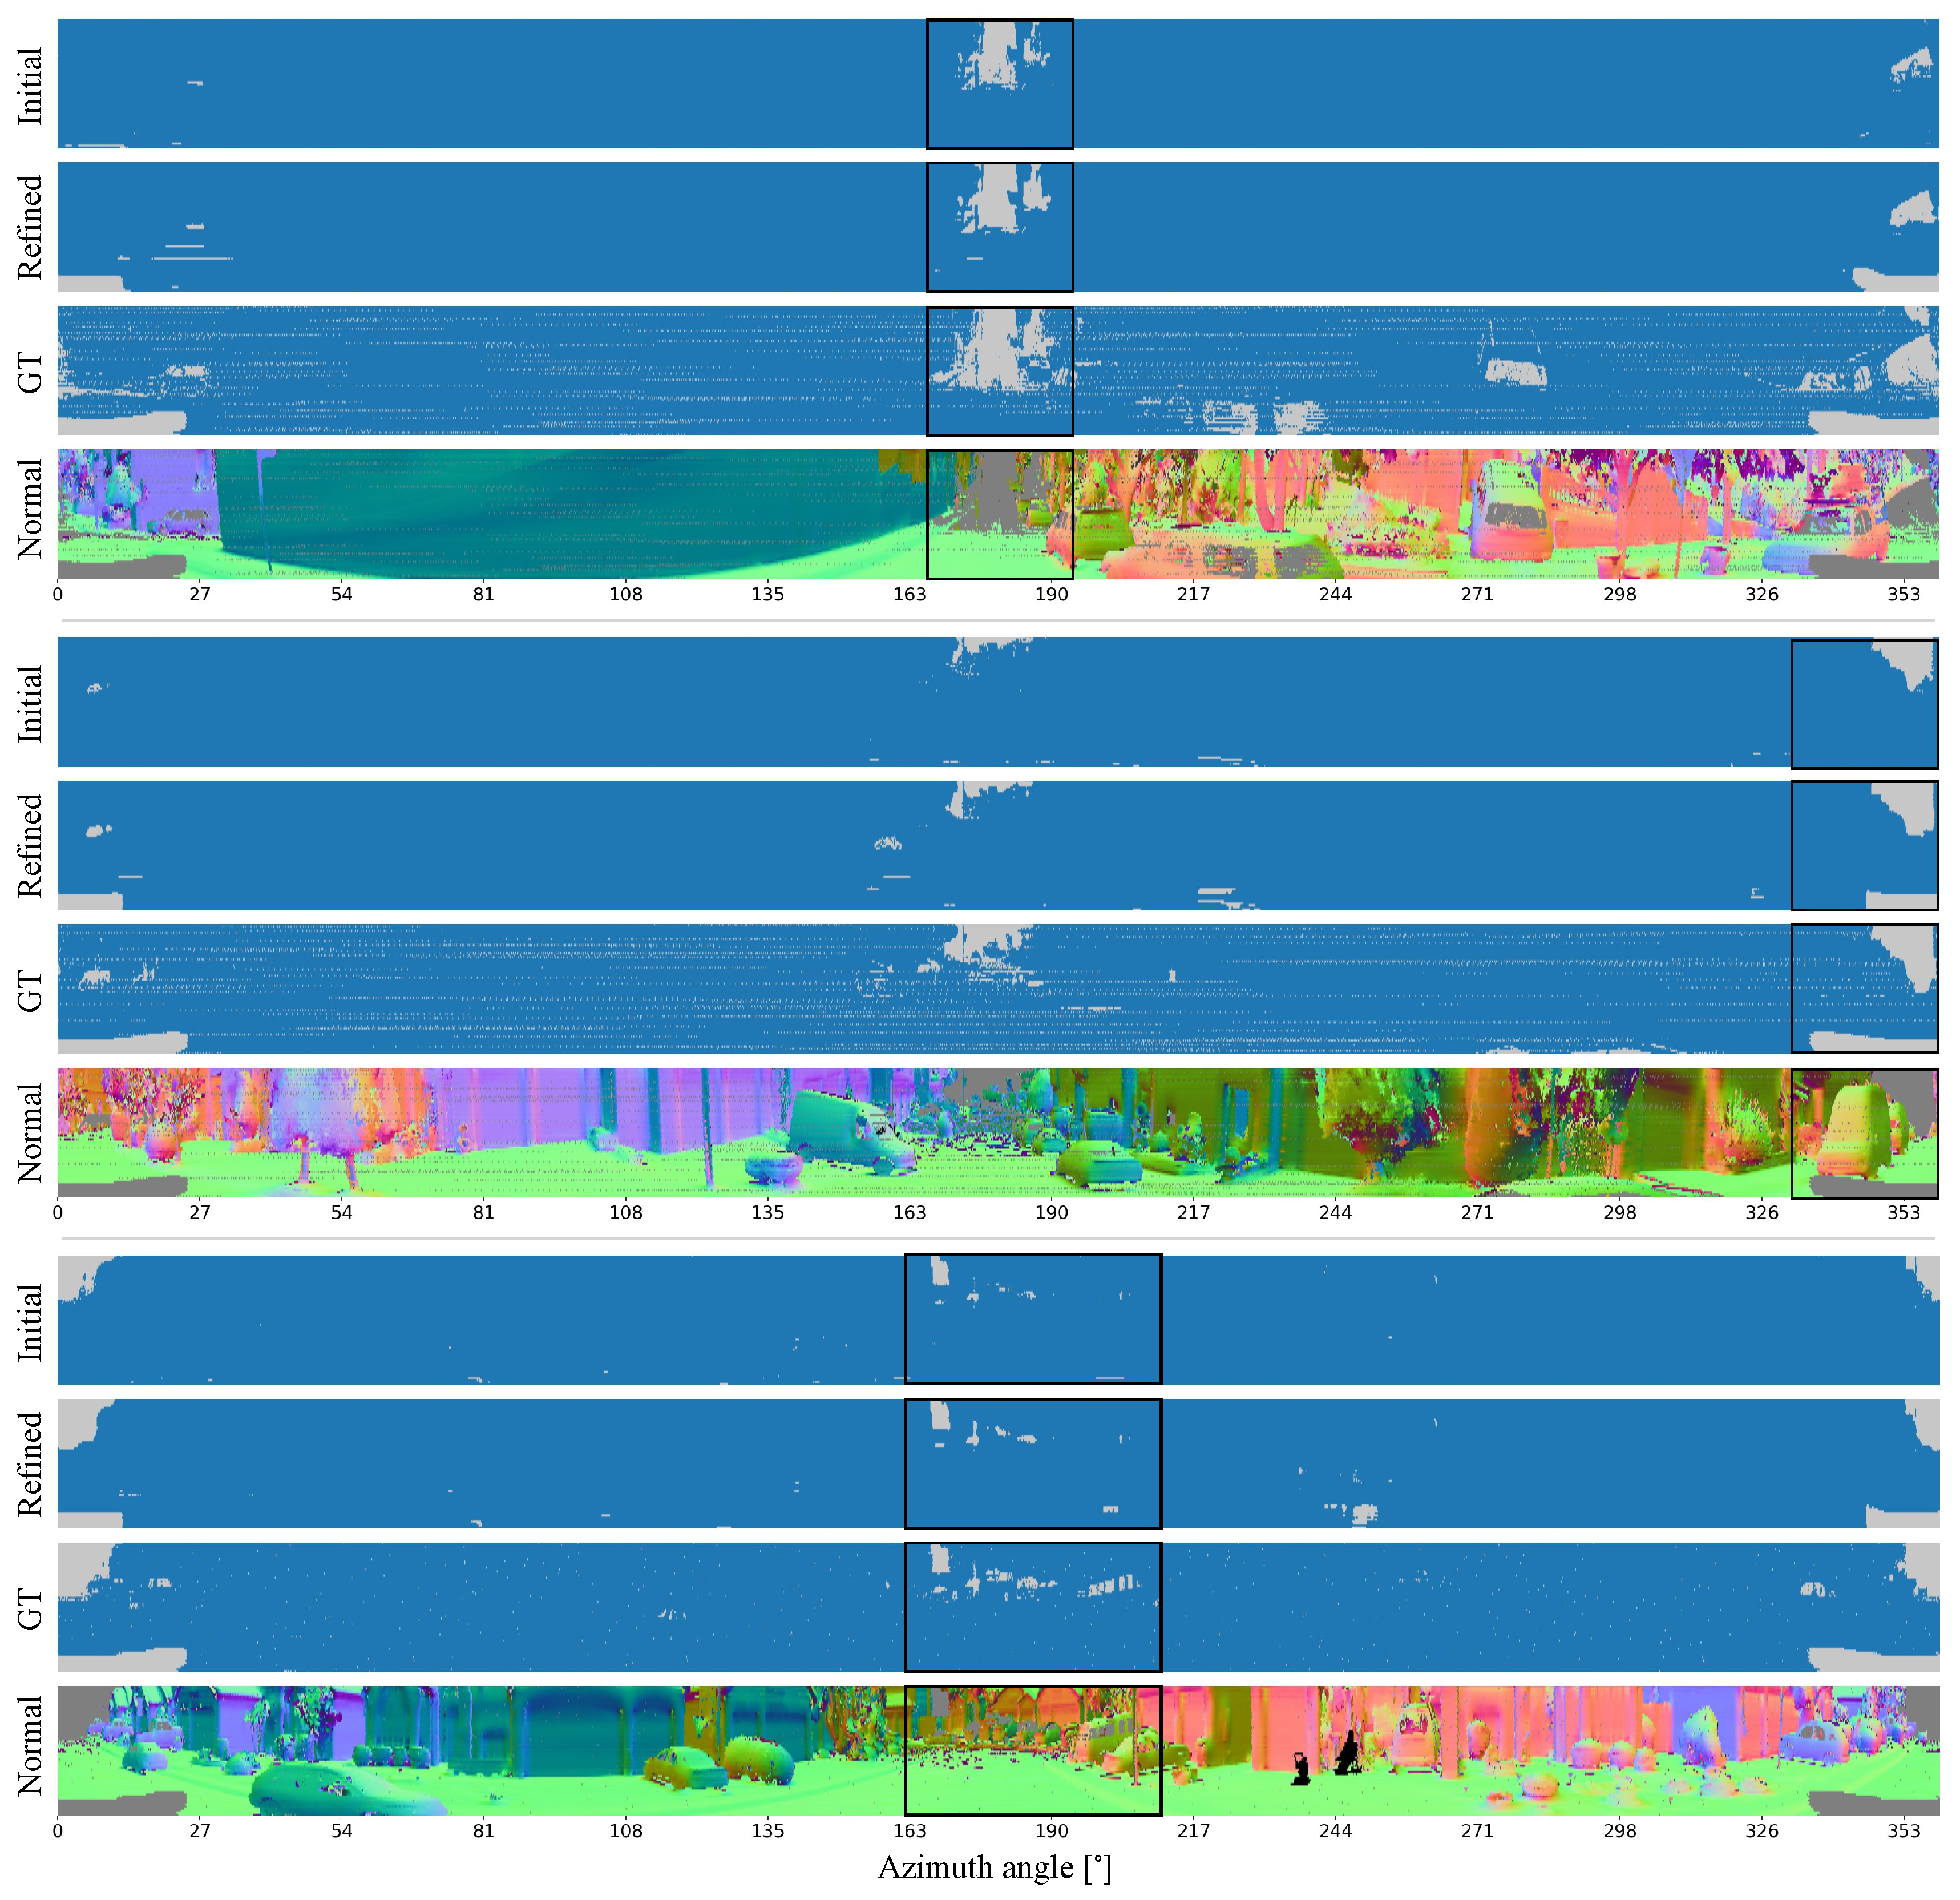
\includegraphics[width=1.0\textwidth]{content/supp/images/lidarsim_ray_drop.pdf}

\caption{Ray drop segmentation on \textit{Waymo Interp.} dataset using LiDARsim~\cite{manivasagam2020lidarsim}. We show both the initial ray drop mask from ray-surfel query and the refined masks using learned ray-drop model.}
\label{fig:supp_lidarsim_raydrop}

\end{figure}
\begin{figure}[t]
\centering
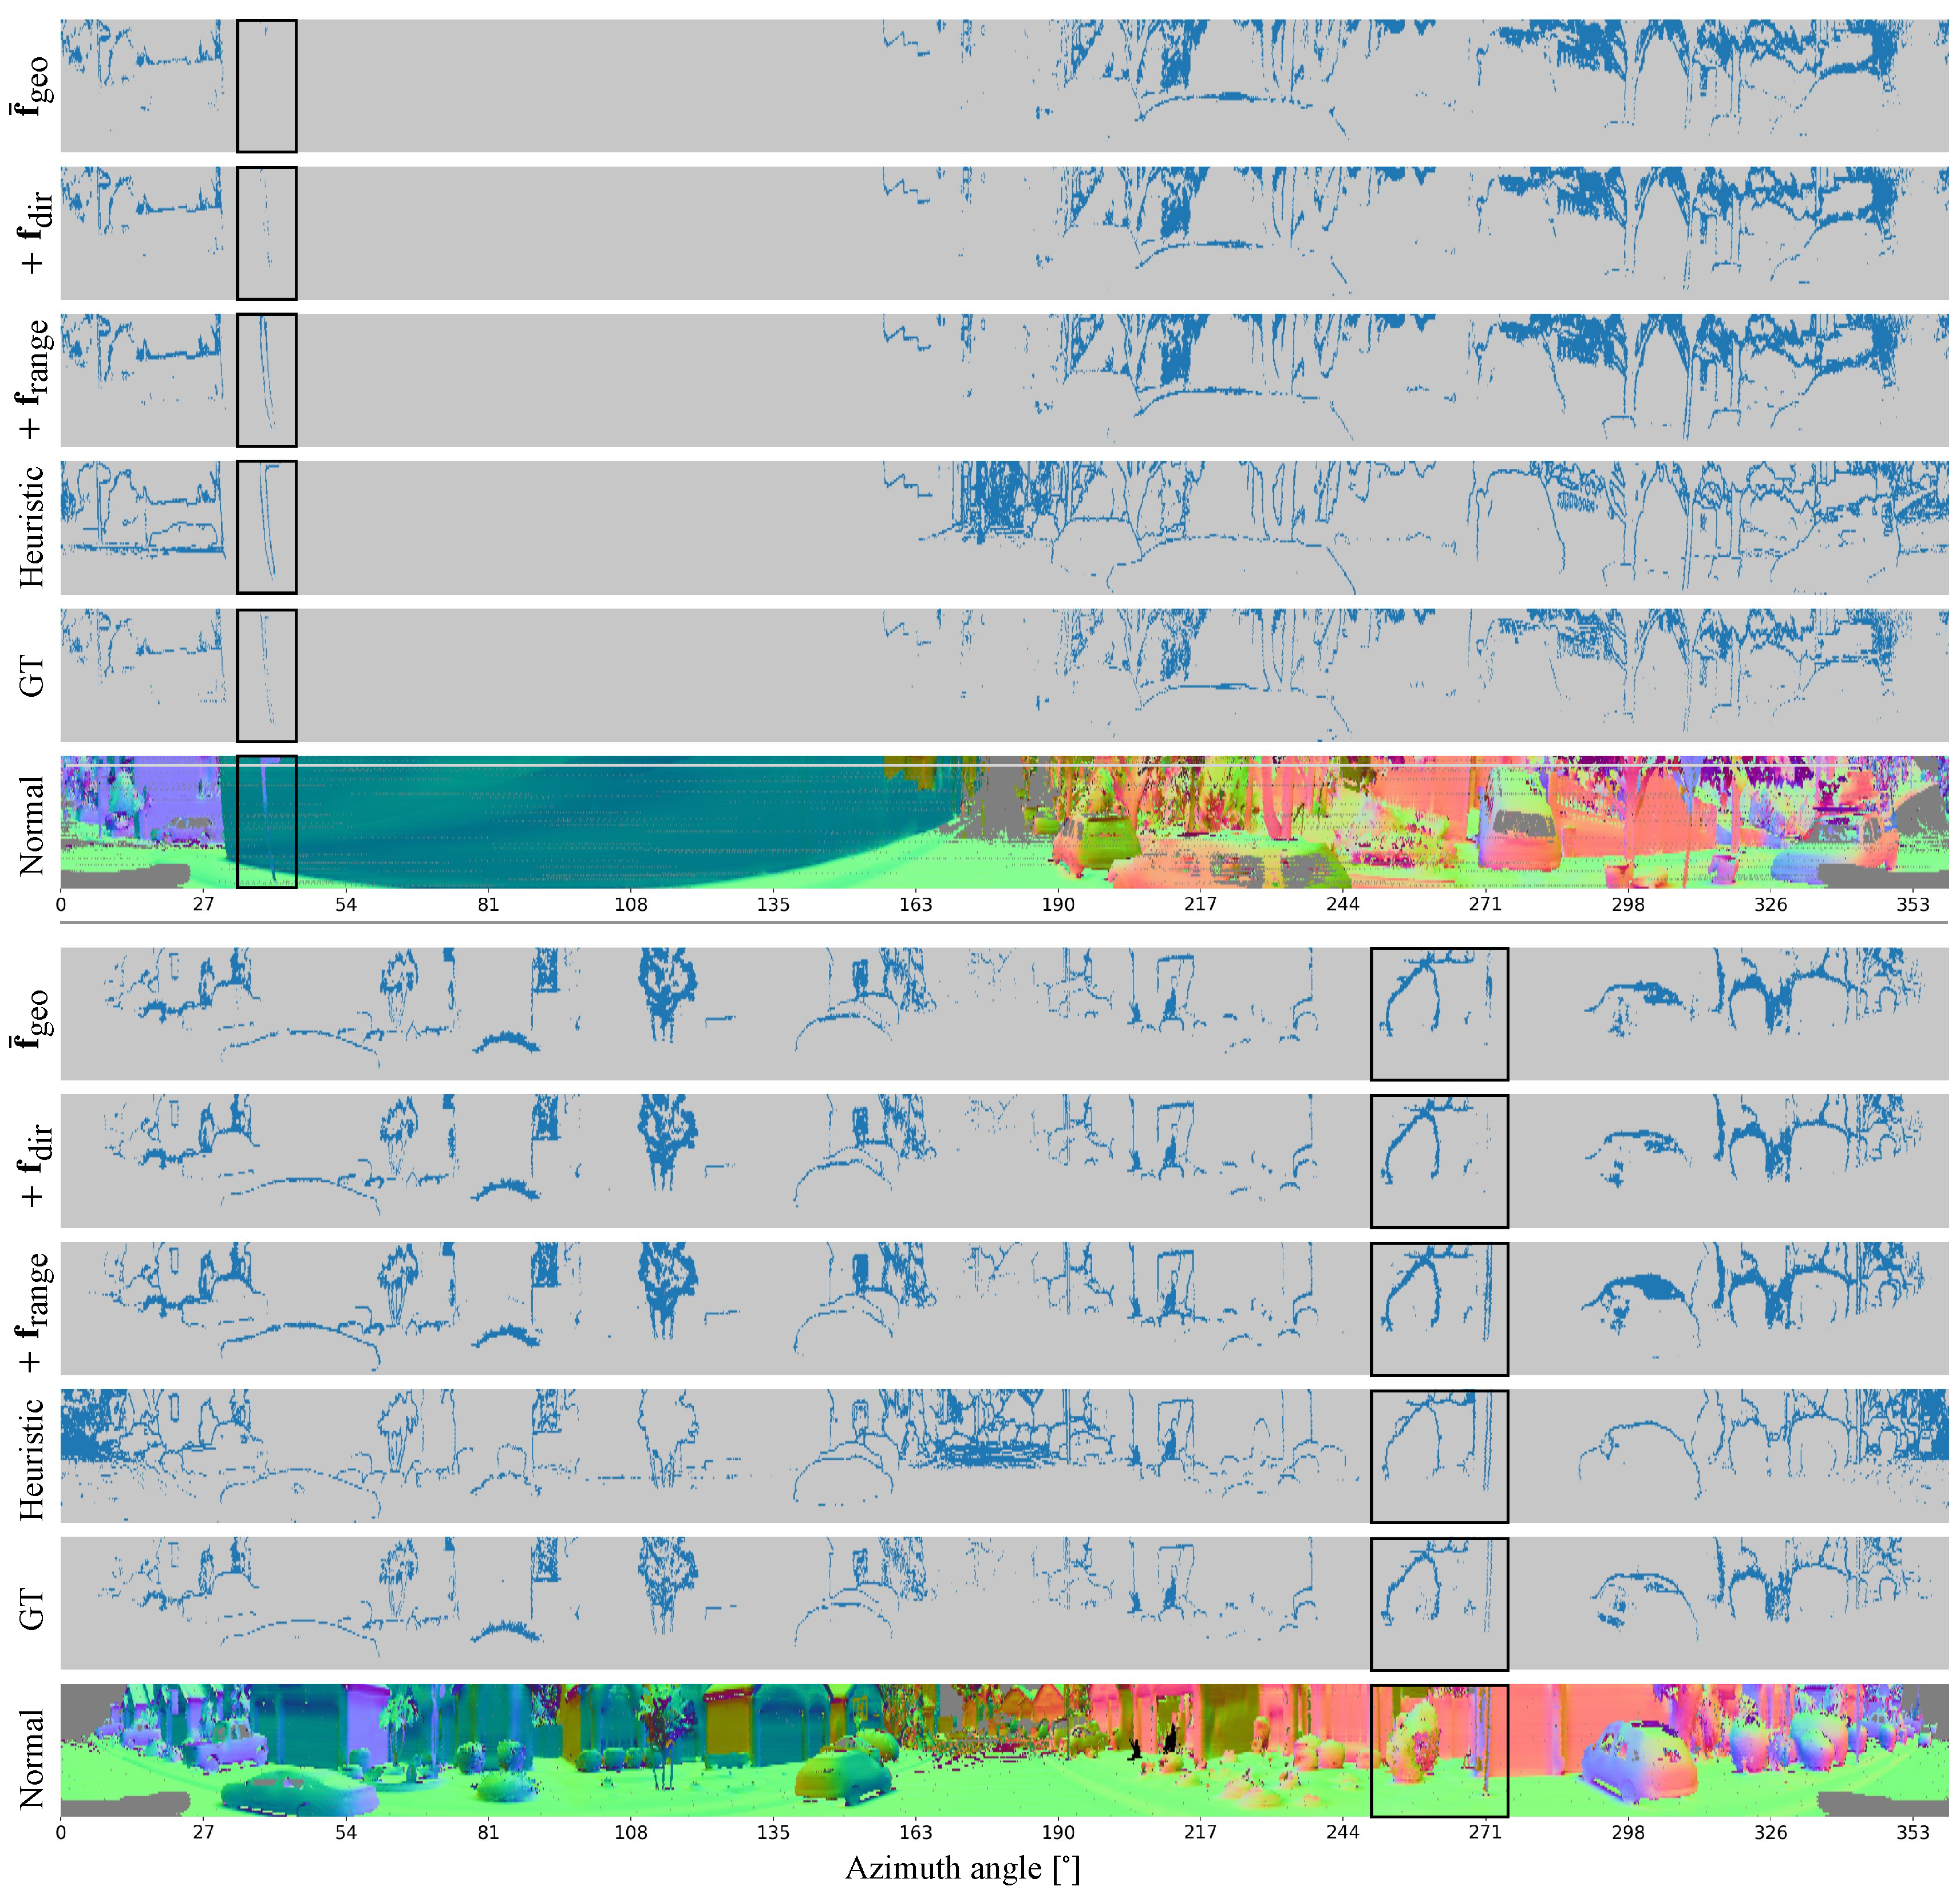
\includegraphics[width=1.0\textwidth]{content/supp/images/ablate_two_return_mask.pdf}

\caption{Qualitative results of two return mask segmentation.}
\label{fig:supp_ablate_two_return_mask}

\end{figure}

\begin{figure}[t]
\centering
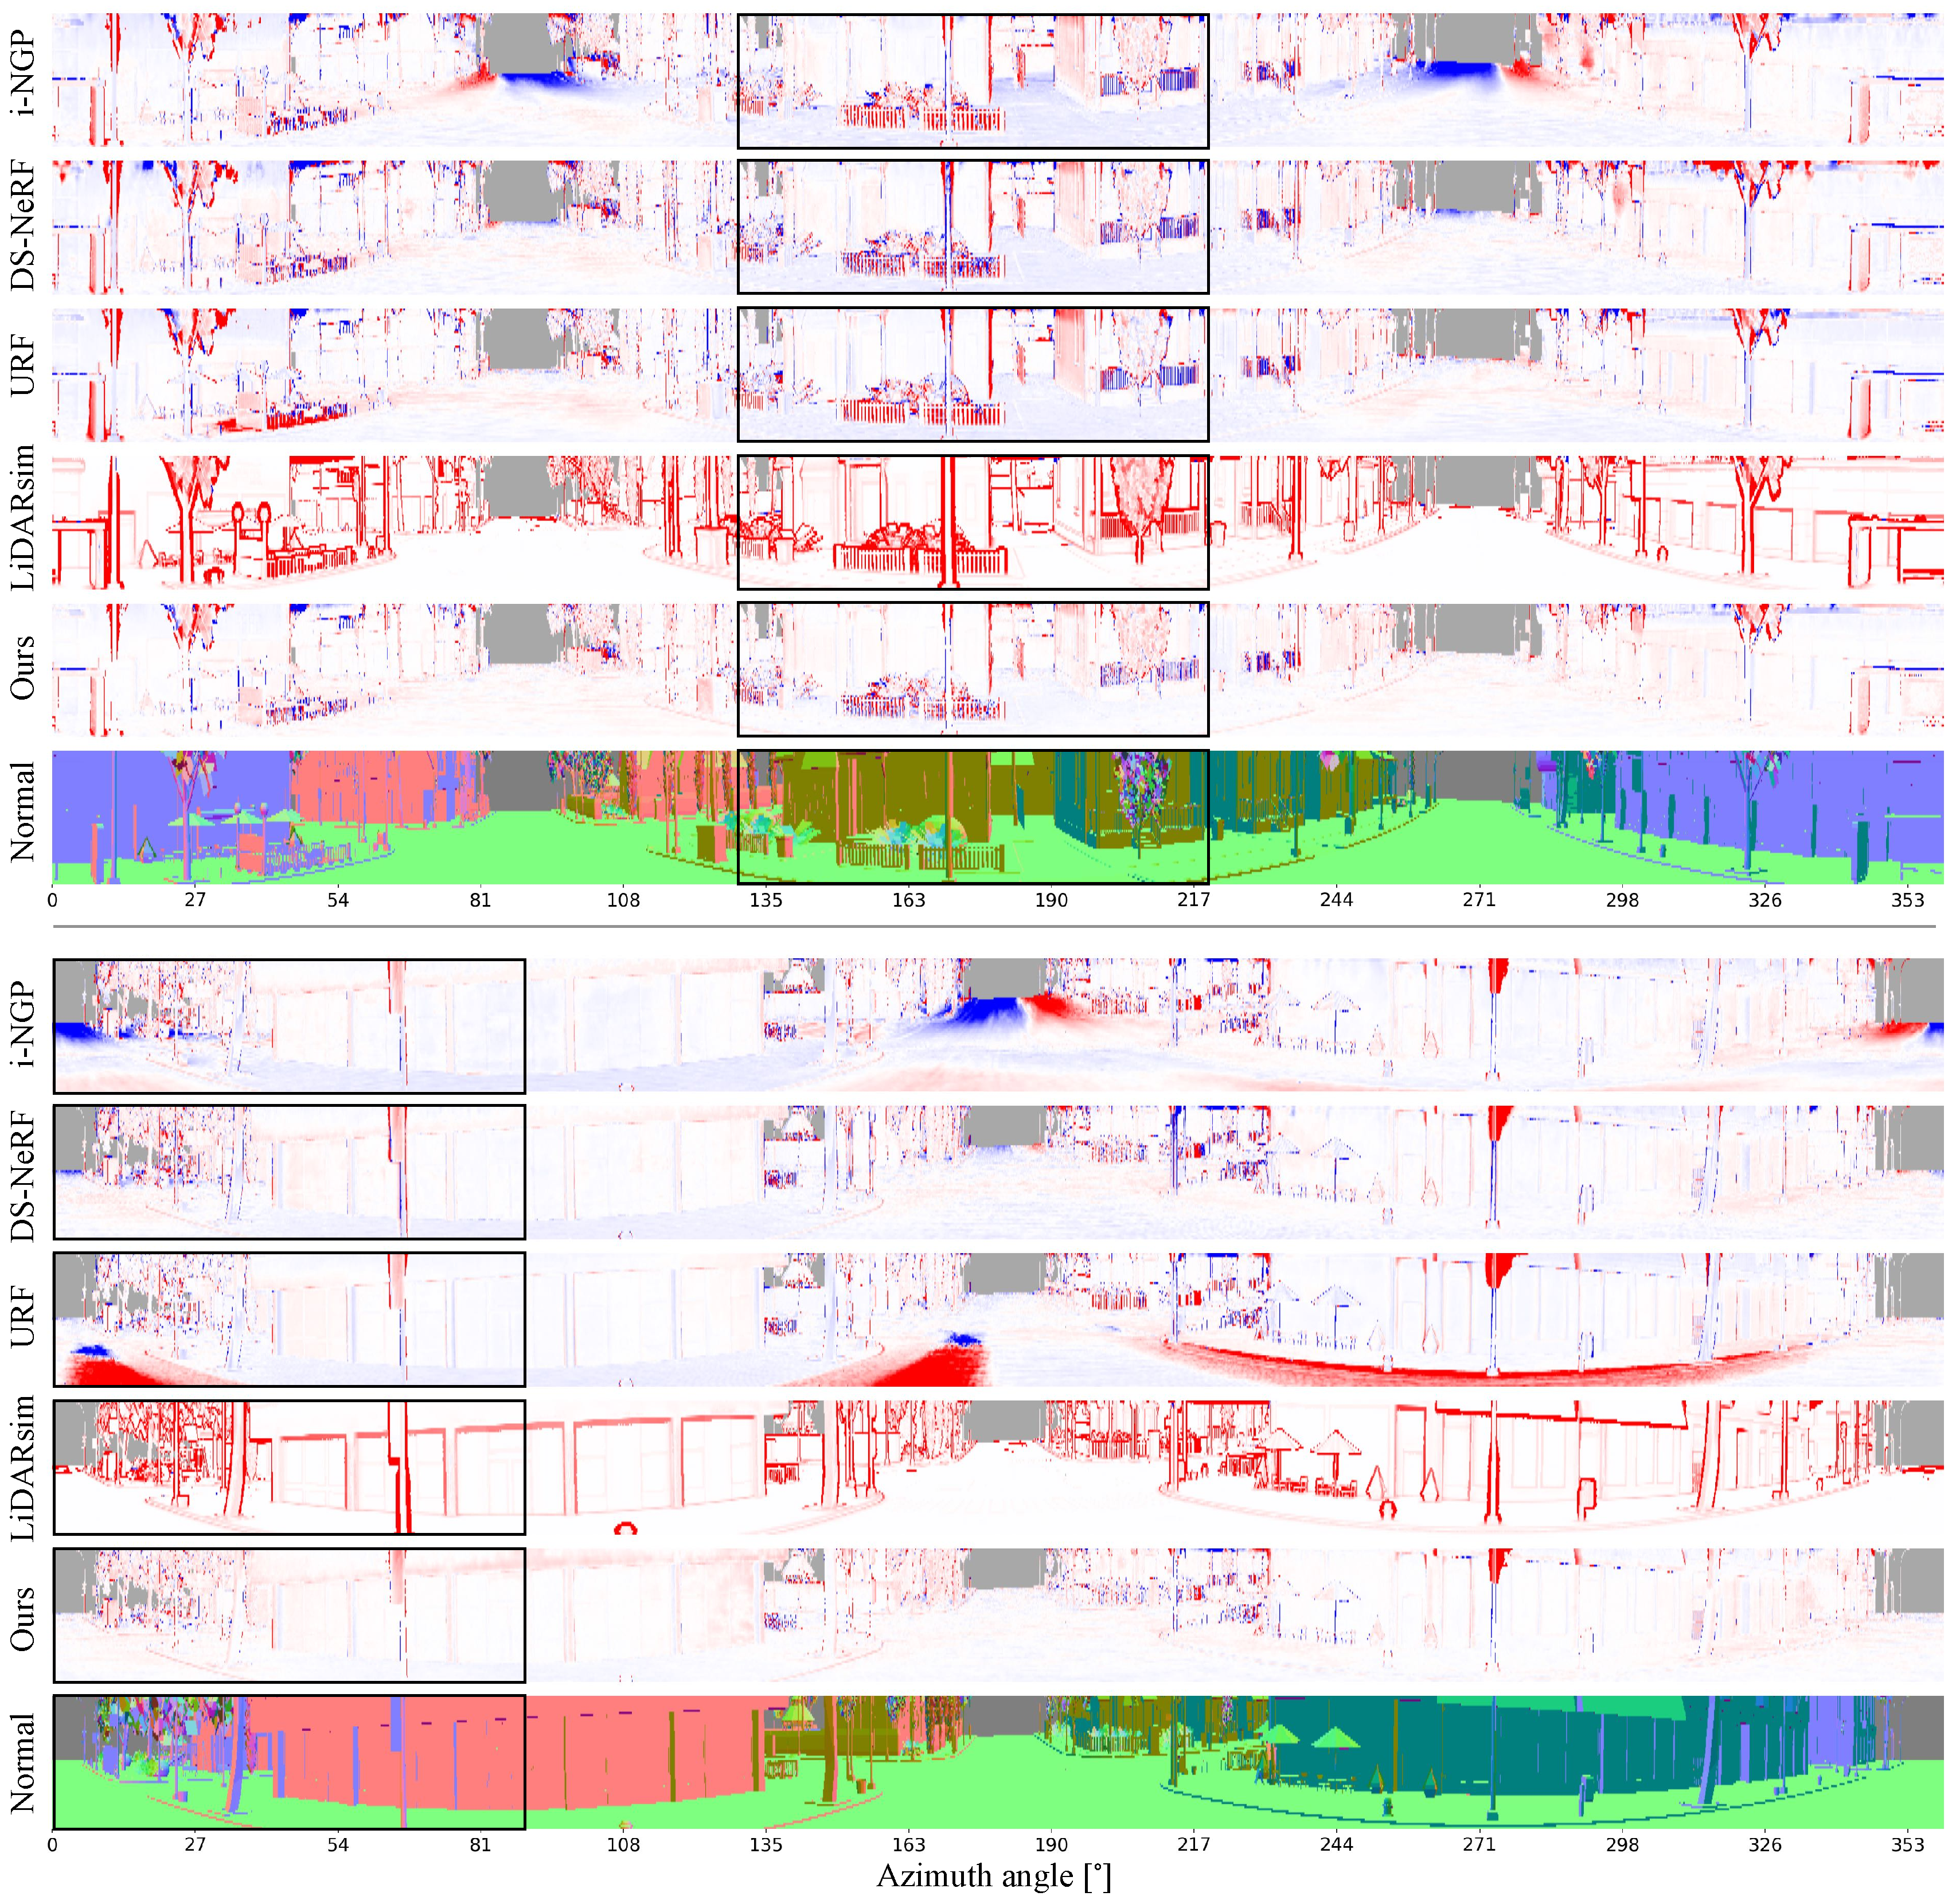
\includegraphics[width=1.0\columnwidth]{supp/images/townclean.pdf}

\caption{Qualitative results of first range estimation on \textit{TownClean} dataset.}
\label{fig:supp_townclean}

\end{figure}
\begin{figure}[t]
\centering
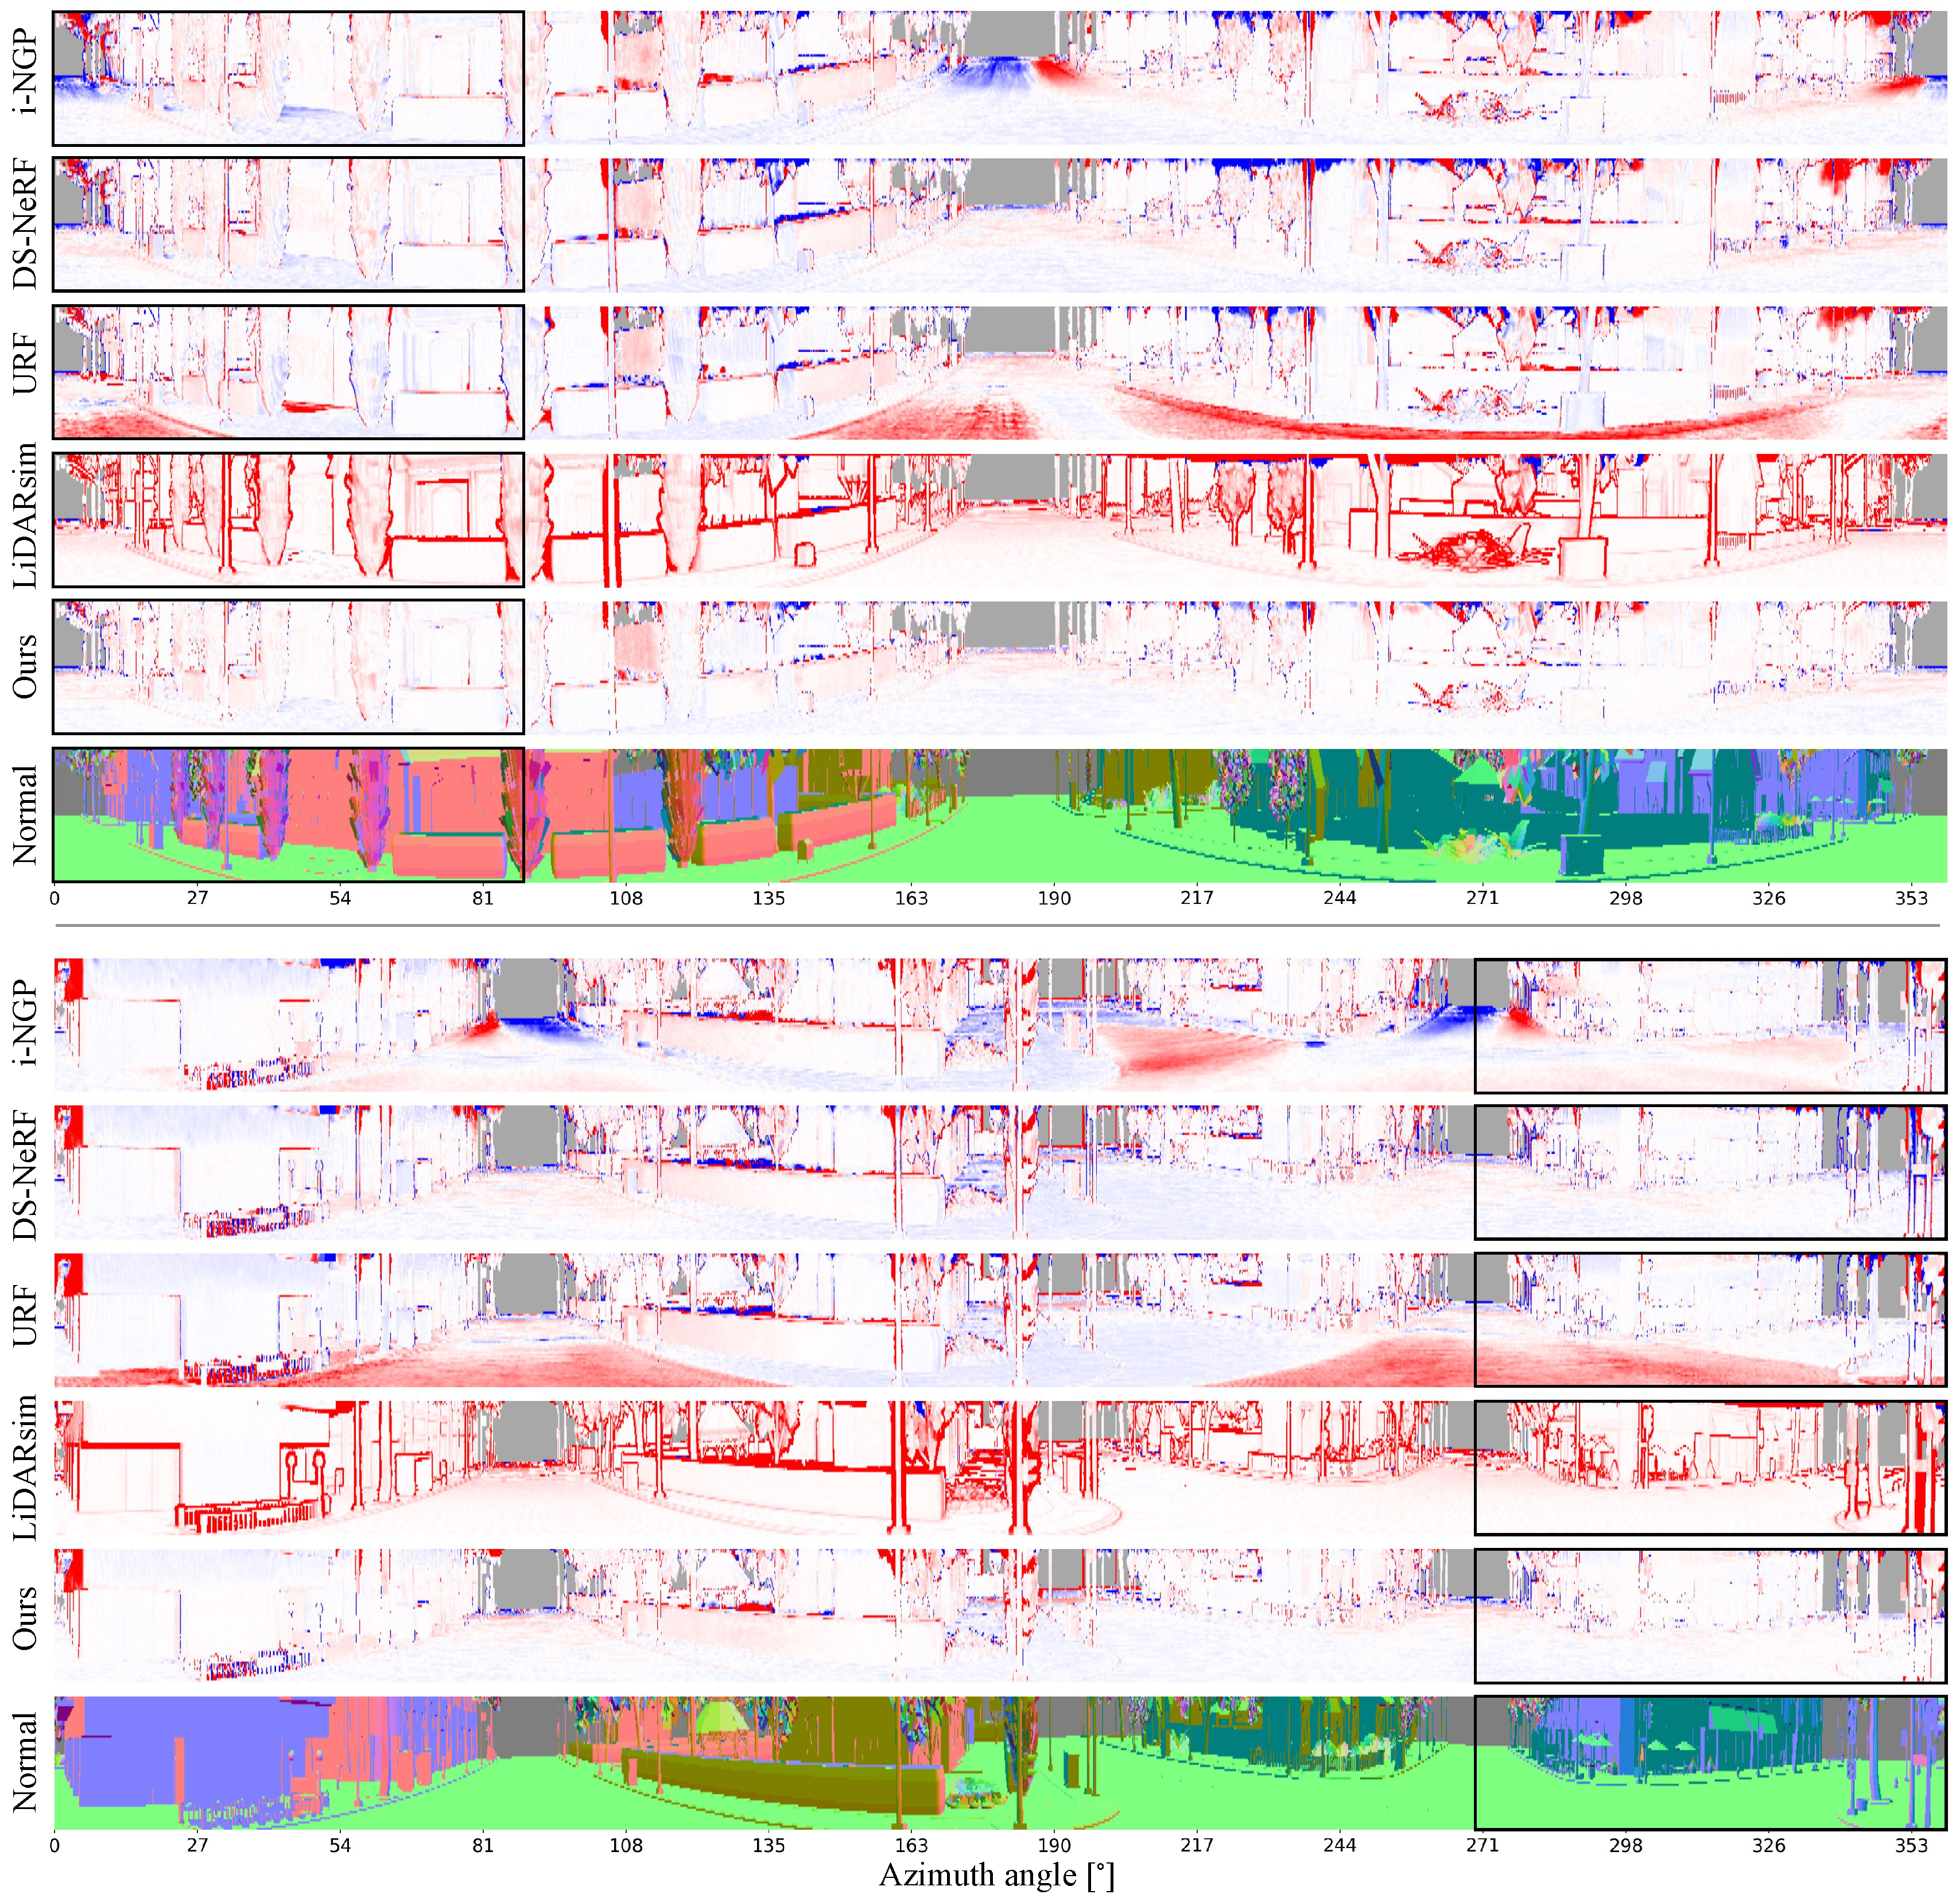
\includegraphics[width=1.0\textwidth]{content/supp/images/townreal.pdf}

\caption{Qualitative results of first range estimation on \textit{TownReal} dataset.}
\label{fig:supp_townreal}

\end{figure}
\begin{figure}[t]
\centering
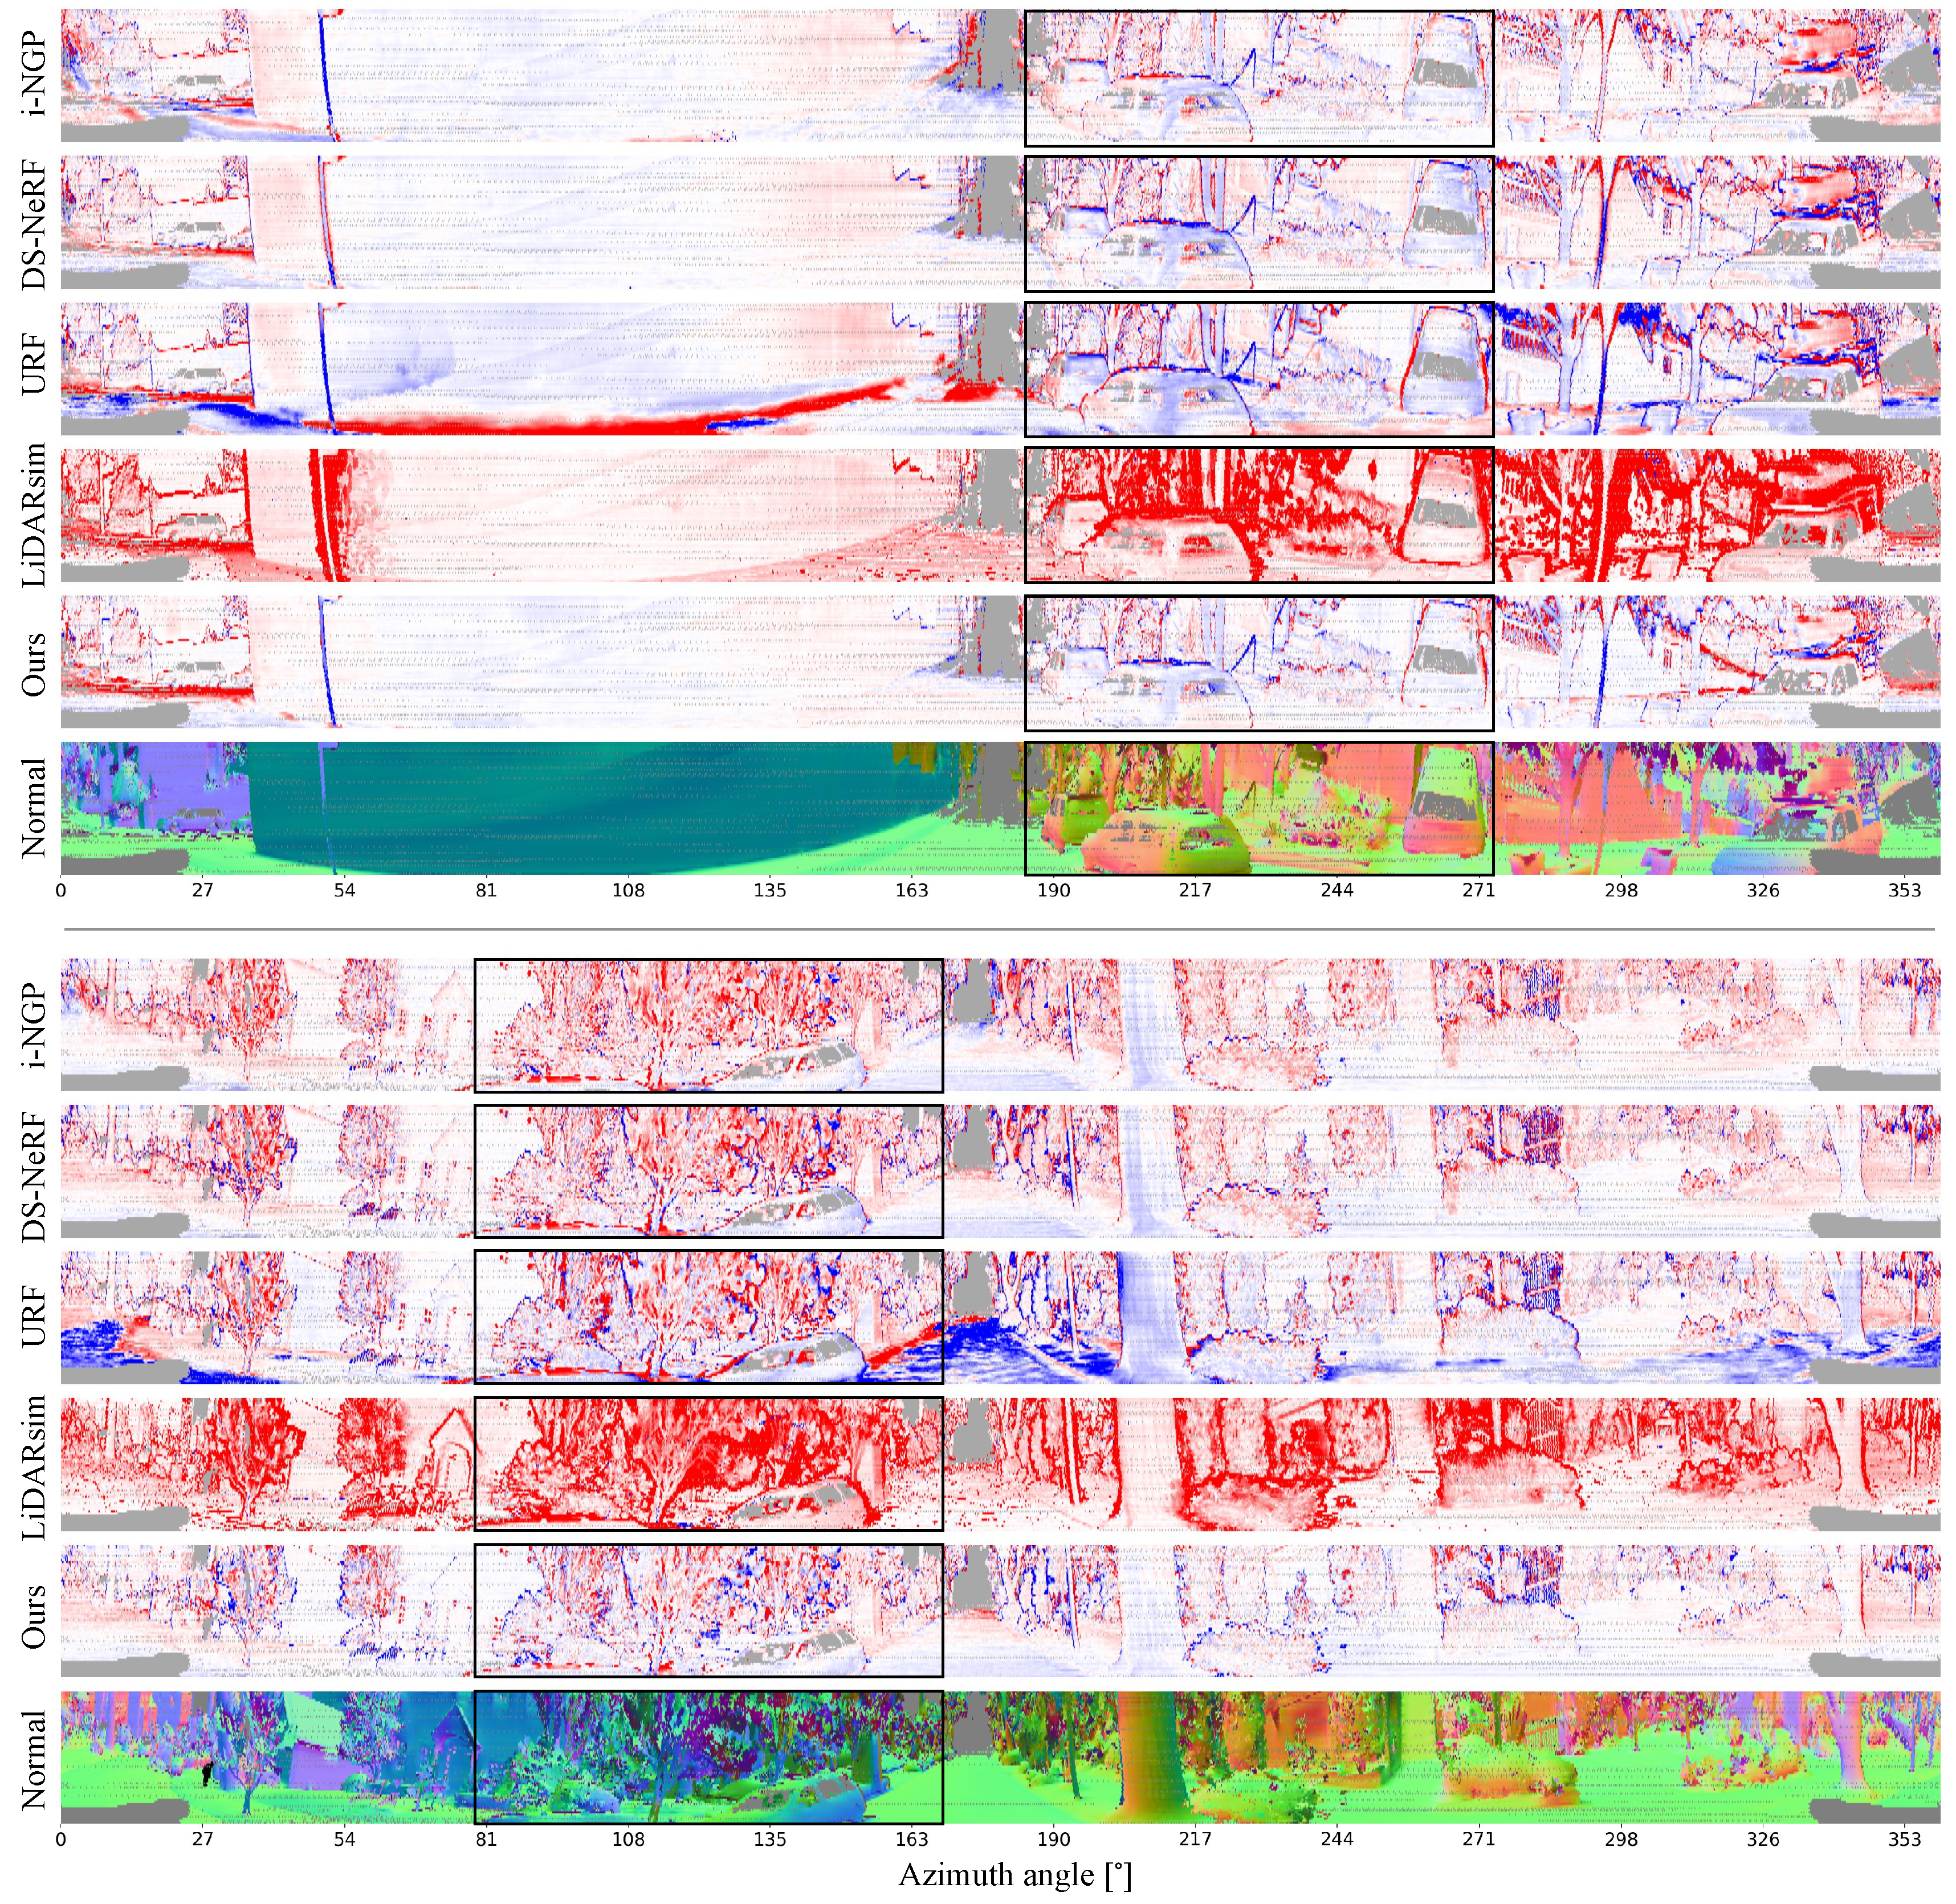
\includegraphics[width=1.0\columnwidth]{supp/images/waymo_nvs.pdf}

\caption{Qualitative results of first range estimation on \textit{Waymo NVS} dataset.}
\label{fig:iccv_supp_waymo_nvs}

\end{figure}
\begin{figure}[t]
\centering
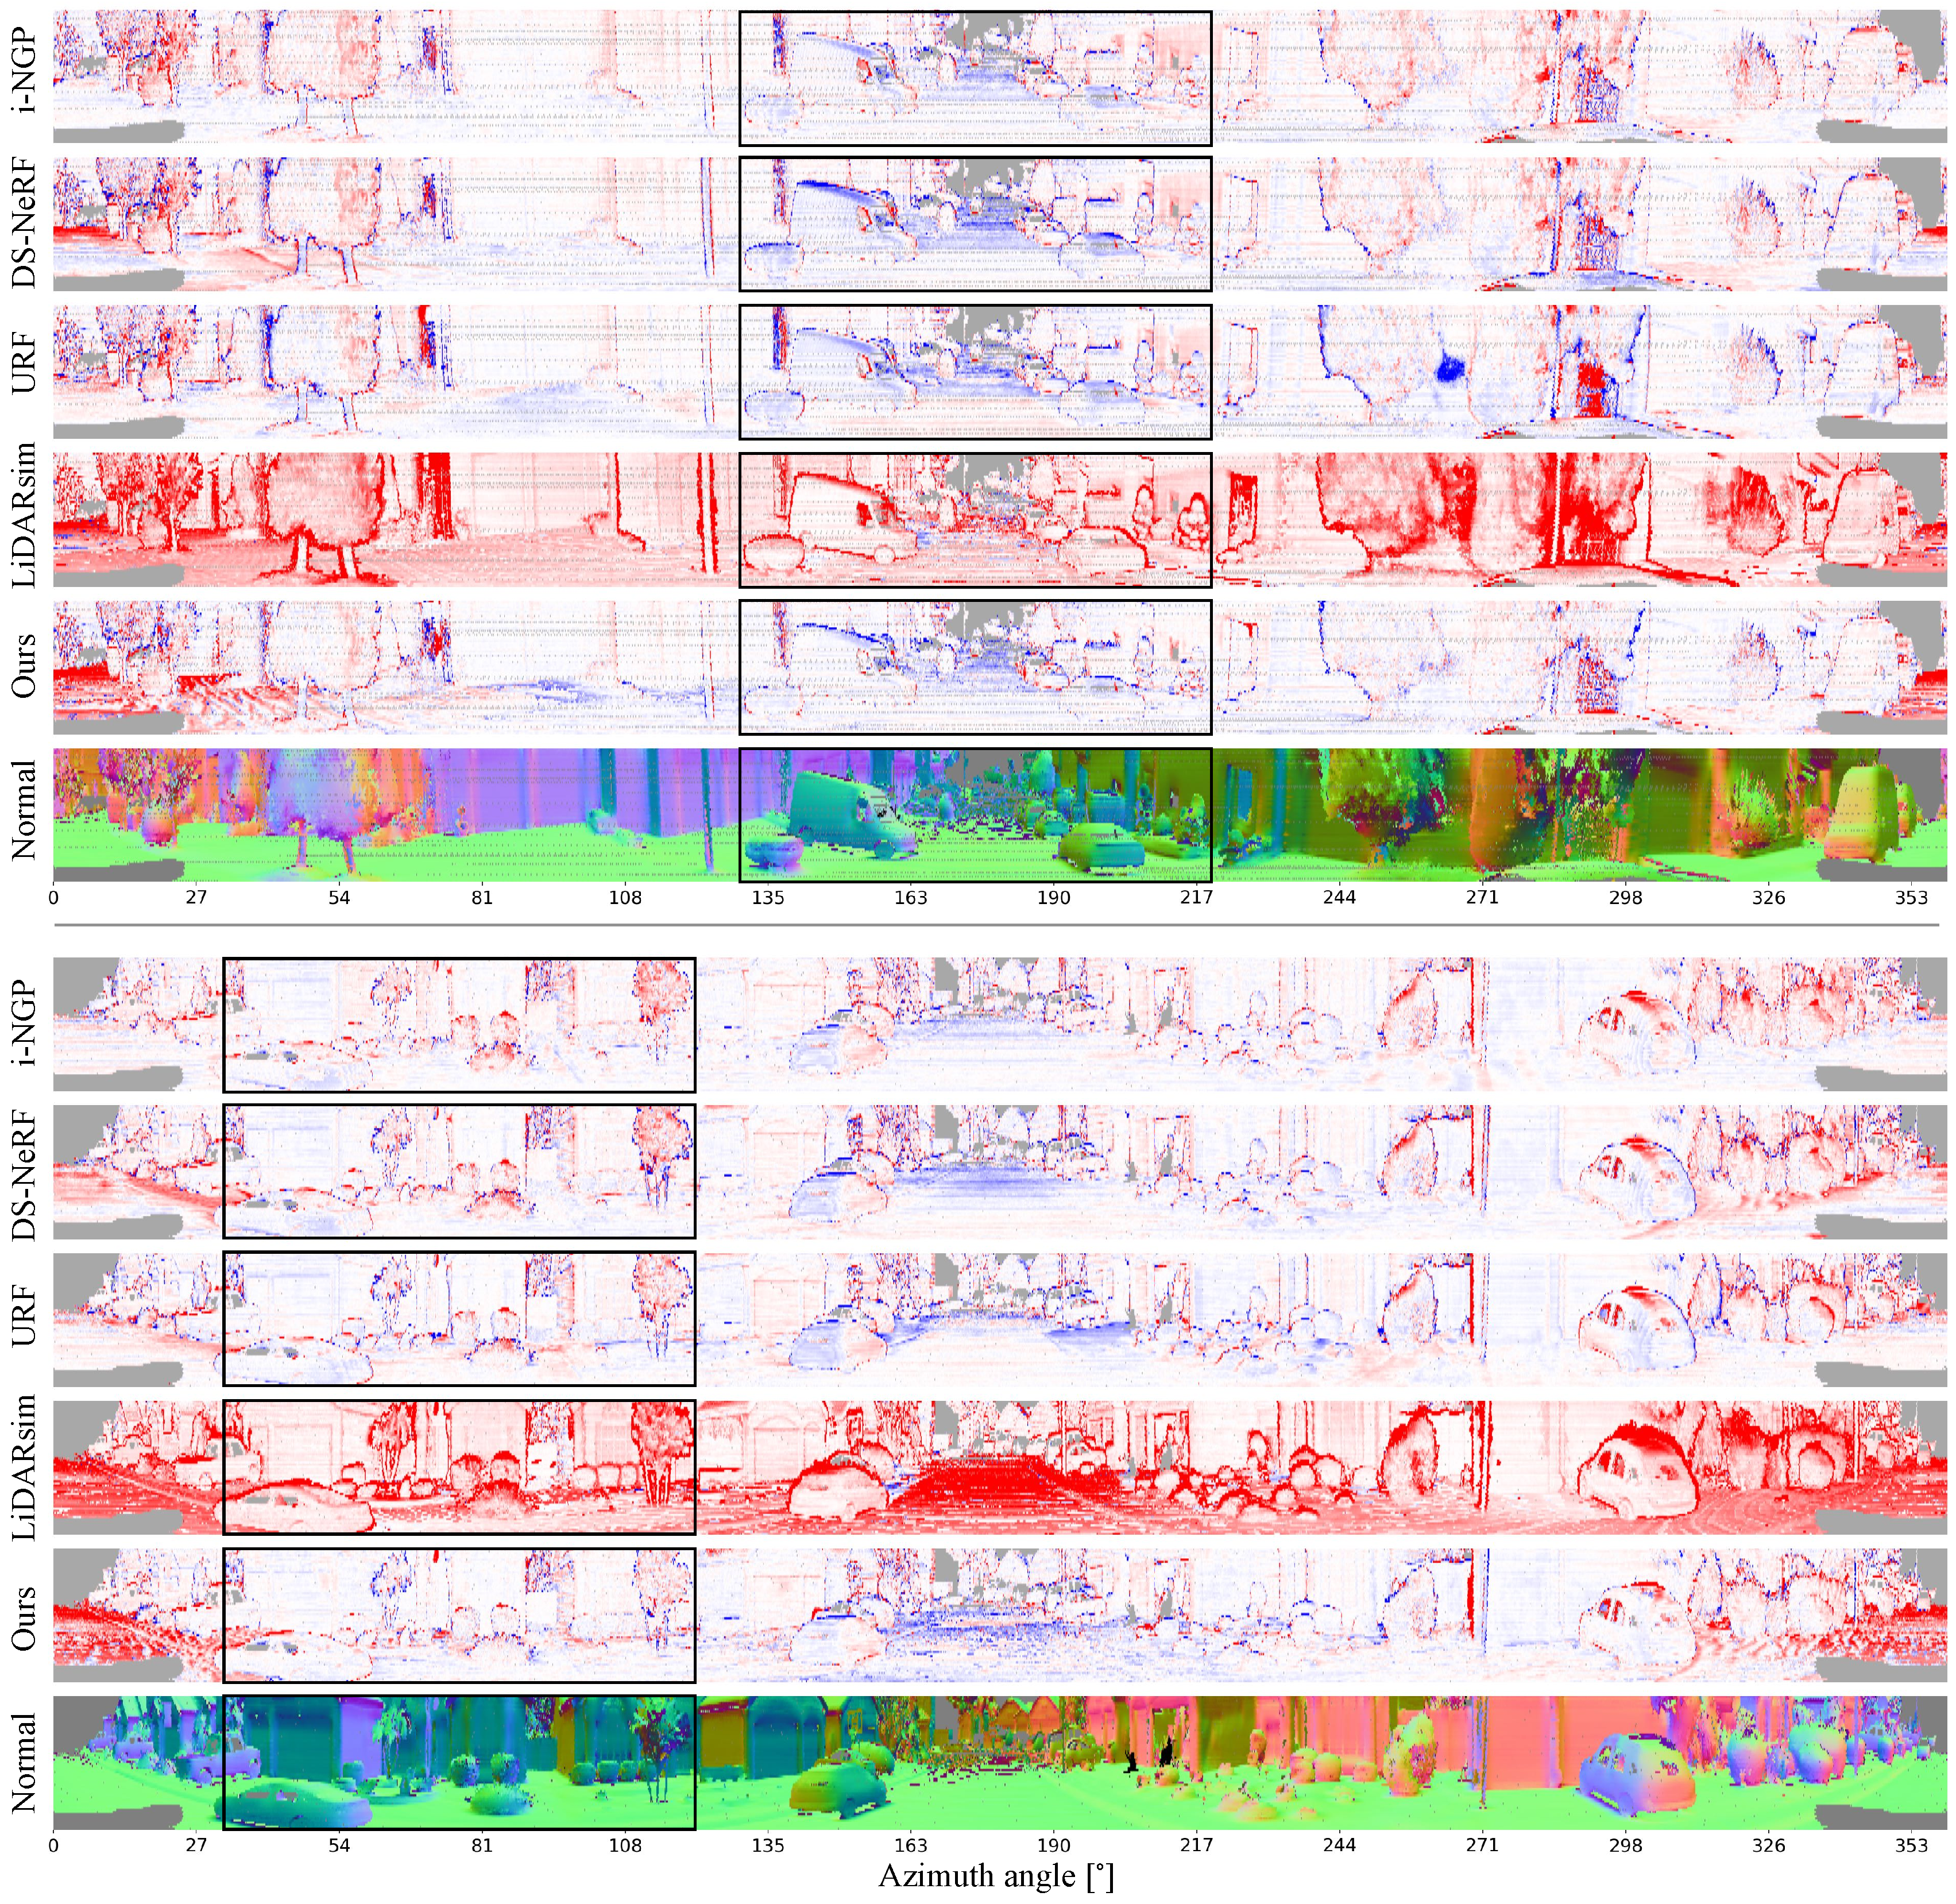
\includegraphics[width=1.0\columnwidth]{supp/images/waymo_interp.pdf}

\caption{Qualitative results of first range estimation on \textit{Waymo Interp.} dataset.}
\label{fig:iccv_supp_waymo_interp}

\end{figure}
